\chapter{Experimental Part}


This chapter presents the practical implementation of modeling and control strategies for a plate heat exchanger, specifically utilizing the Armfield Process Plant Trainer PCT23 \cite{armfield_pct23_manual}. It details the procedures for system identification, controller design, and performance evaluation through both simulation and real-time experimentation. The approach throughout closely follows established practices in process control \cite{ljung_sysid, rawlings_mpc}, while adapting recent data-driven modeling techniques where appropriate.

\section{The Plate Heat Exchanger}
\label{sec:practical_introduction}
The Armfield PCT23 is a laboratory-scale plate heat exchanger with two hydraulically separated circuits: a hot-fluid circuit and a cold-fluid circuit. Heat transfer between the two media takes place in the plate heat exchanger, while the overall process dynamics are influenced by the flow rates and inlet temperatures of both circuits. The system exhibits slow dynamics and nonlinear behavior typical of thermal processes.

\begin{figure}[htbp]
    \centering
    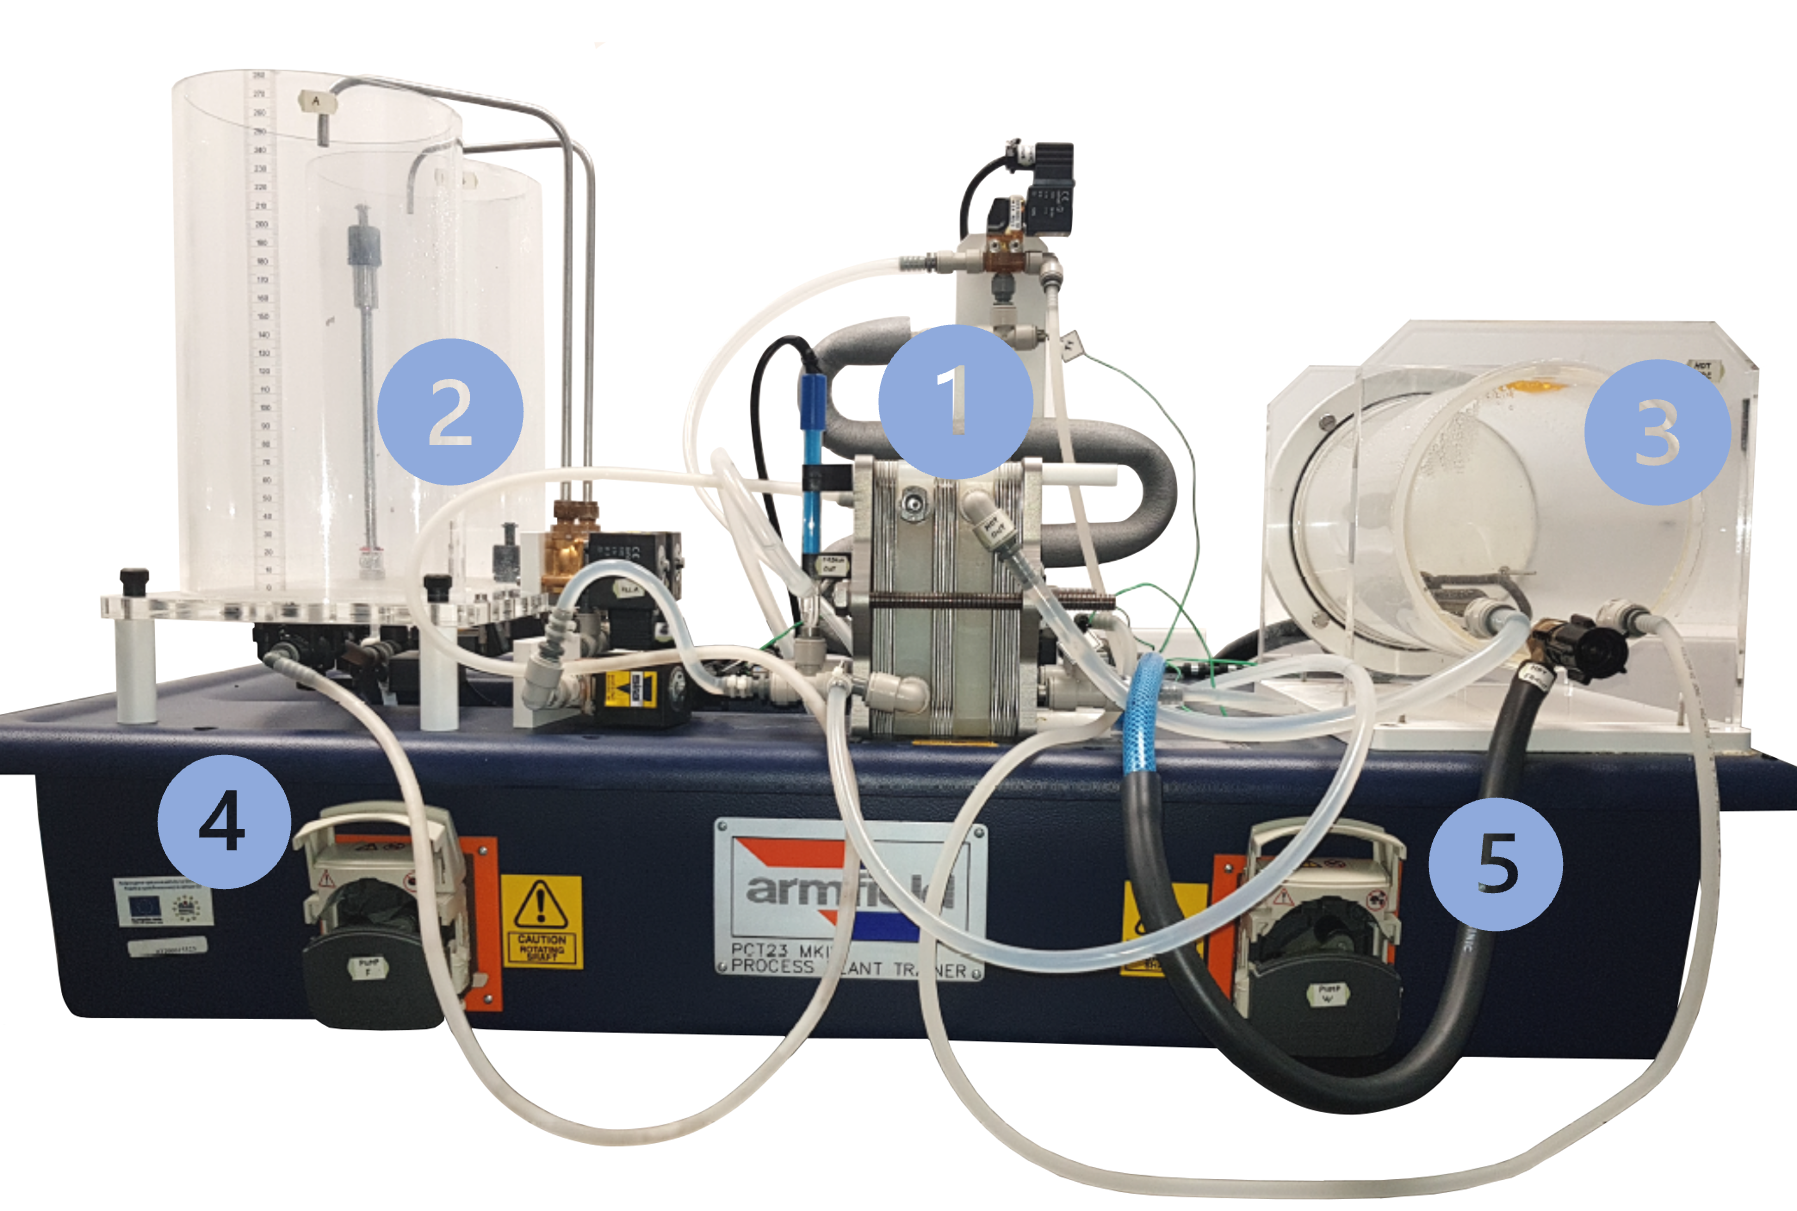
\includegraphics[width=0.6\textwidth]{images/PU.png}
    \caption{Armfield Process Plant Trainer PCT23. (1) Plate heat exchanger, 
    (2) cold water reservoir, 
    (3) hot water reservoir with electric heating, 
    (4) Pump~W for the cold water circuit, 
    (5) Pump~F for the hot water circuit.}
    \label{fig:pct23_plant}
\end{figure}

The hot medium is heated by an electric heater, whose power is regulated by a dedicated P controller to maintain the inlet temperature of the hot circuit at an approximately constant 76$^\circ$C. In this work, the heater control is treated as an auxiliary control loop and is not included in the main control design.

The experimental setup is shown in Figure~\ref{fig:pct23_plant}. The plate heat exchanger is indicated by label~(1). The hot water circuit is driven by the heating pump (component~(5), which supplies heated water to the heat exchanger. The remaining components include the hot and cold water reservoirs and the corresponding circulation pumps.

The system is treated as a SISO system with the outlet temperature from the heat exchanger, denoted as $T_4$, as the controlled output and the pump power of the hot circuit, denoted as Pump~F, as the manipulated input. The pump power directly affects the flow rate and, consequently, the heat transfer rate. The control input is constrained by the physical limits of the pump within the range of $20$--$100~\%$. The pump for the cold liquid was kept constant at $50~\%$.


The main aim of the practical part is to identify suitable models of the heat exchanger process from experimental data, design MPC controllers using both a classical first-order model and a data-driven Koopman model, and compare their closed-loop performance under identical constraints in both simulation and real-time operation on the PCT23 system. This comparative methodology has been widely adopted in recent literature for benchmarking advanced control strategies \cite{benchmark_mpc2021}.



\section{System Identification}

System identification experiments were conducted to collect input–output data for developing both classical and data-driven models of the heat exchanger. All experiments were performed on the Armfield PCT23 setup. The identification process follows standard procedures outlined in system identification textbooks \cite{ljung_sysid}.

Before the identification measurements, the heat exchanger was operated until steady conditions were achieved. The temperature of the hot circuit was regulated by the built-in electric heater, whose power was controlled by a simple proportional controller. The controller gain was selected to maintain the inlet temperature of the hot circuit close to a steady-state value. Throughout all identification experiments, the heater control settings were kept unchanged to ensure consistent thermal conditions. This auxiliary control loop was not modified and is therefore not considered part of the identification process.

During the identification experiments, the pump supplying the hot circuit (Pump~F) was used as the manipulated input. The pump speed was changed in steps every $250~\mathrm{s}$ to capture the system's dynamic response.

The pump of the cold circuit (Pump~W) was operated at a constant speed of $50~\%$ throughout the experiments. This ensured a steady flow rate of the cold medium and allowed the hot flow rate to be isolated from the outlet temperature.

The measured output used for identification was the temperature at the outlet of the heat exchanger, denoted as $T_4$. The pump speed and the corresponding outlet temperature were recorded continuously. Figure~\ref{fig:raw_measurements} shows the applied input signal (Pump~F speed) and the resulting outlet temperature response used for system identification.

\begin{figure}[htbp]
    \centering
    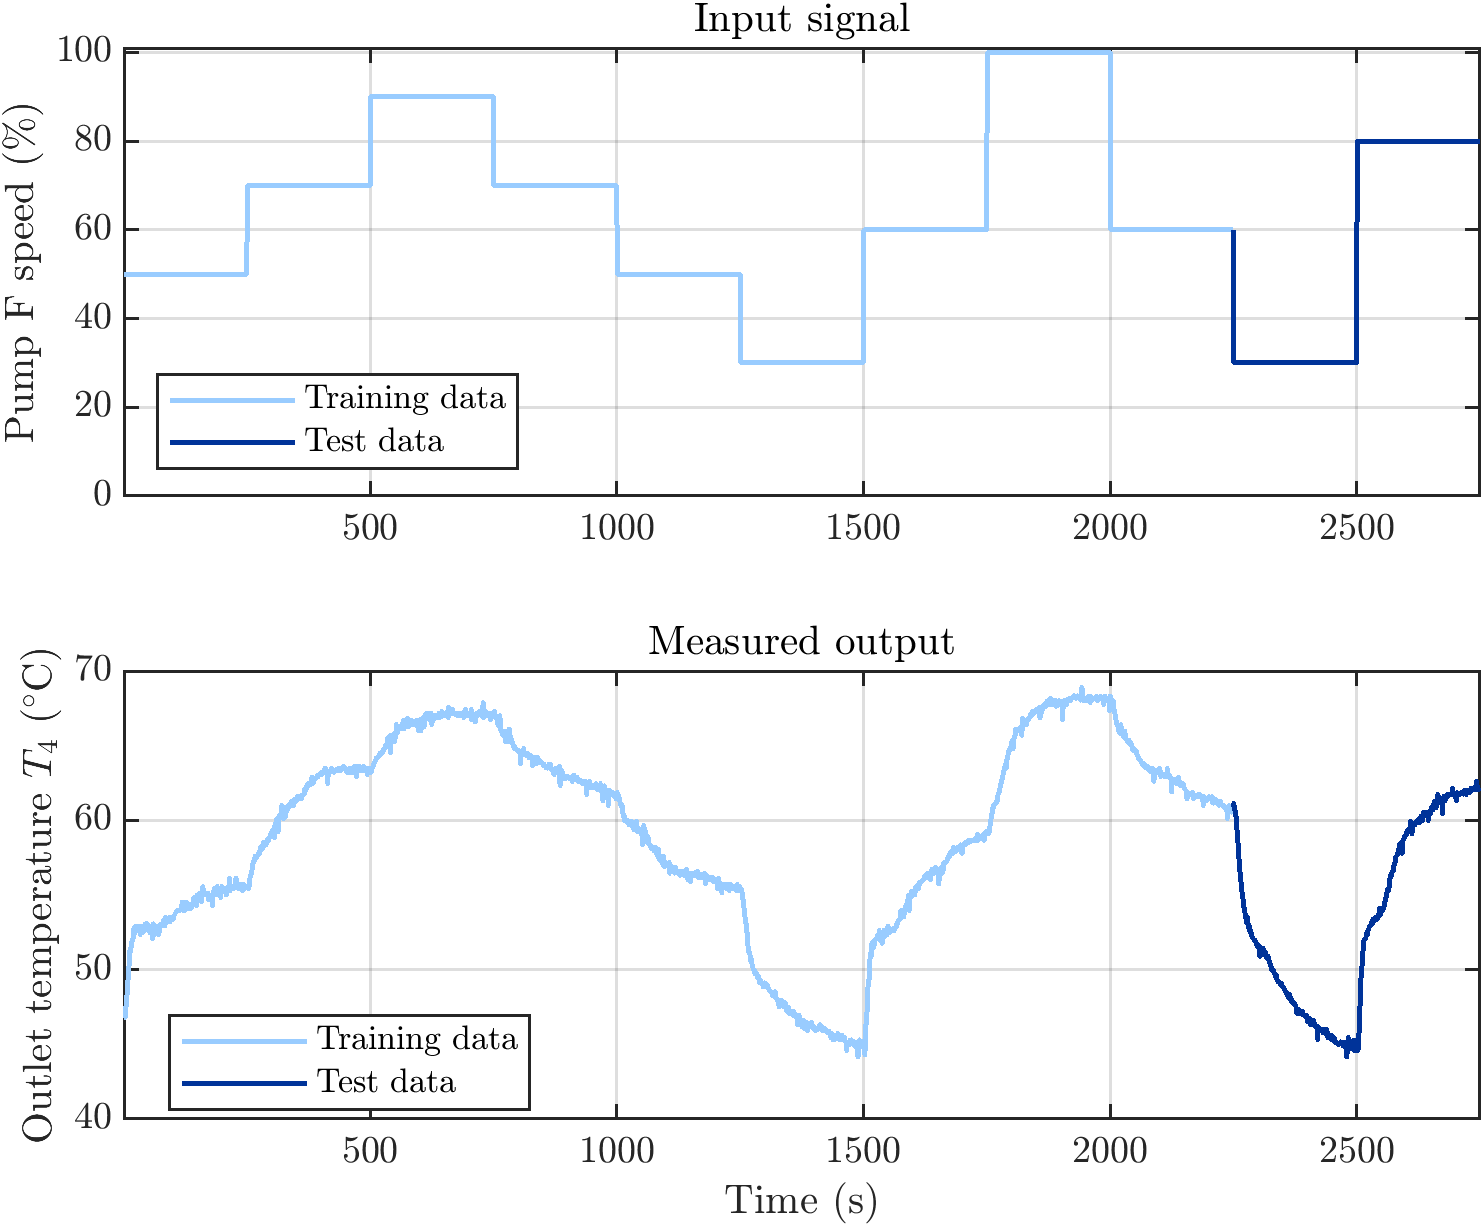
\includegraphics[width=\textwidth]{images/raw_identification_measurements.png}
    \caption{Measured input signal (Pump~F speed) and measured outlet temperature $T_4$ used for system identification.}
    \label{fig:raw_measurements}
\end{figure}

For comparison of responses obtained at different operating points, the measured signals were centered using their empirical mean values,
\begin{equation}
\bar{y} = \mathrm{mean}(y) = 59.07\,^{\circ}\mathrm{C}, \qquad
\bar{u} = \mathrm{mean}(u) = 65.84\,\%.
\end{equation}
These values were also used for the step response analysis.

Step responses were extracted from the measured data by detecting changes in the input signal. The corresponding temperature responses were aligned in time and scaled according to the input step size. The normalized step responses are shown in Figure~\ref{fig:normalized_steps}. Minor differences between individual responses are present, but the dominant dynamics are consistent.

\begin{figure}[htbp]
    \centering
    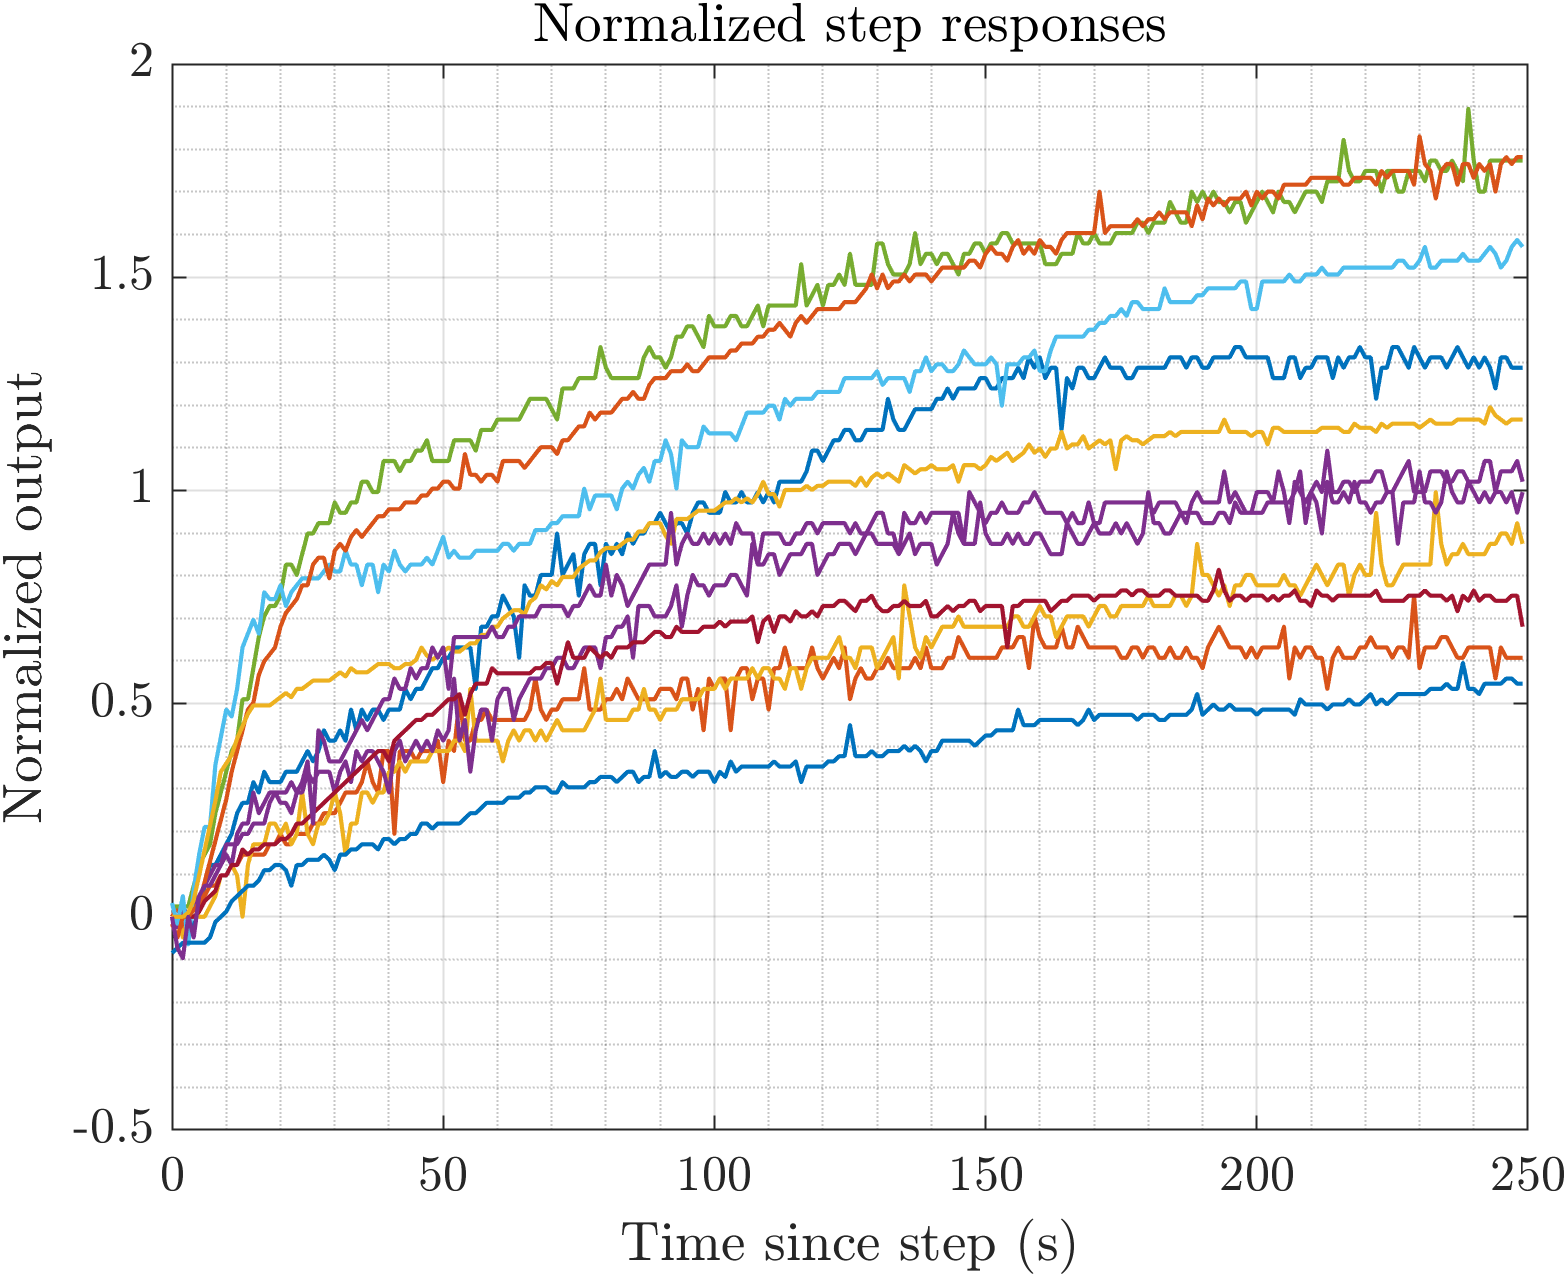
\includegraphics[width=0.8\textwidth]{images/fig_normalized_step_responses.png}
    \caption{Normalized step responses of the outlet temperature $T_4$ to step changes in Pump~F speed.}
    \label{fig:normalized_steps}
\end{figure}

\subsection{First-order Linear Identification of the Heat Exchanger}
\label{sec:strejc_ident}

An average normalized step response was obtained by averaging all valid normalized responses from the identification dataset. This averaged response provides a representative description of the dominant process dynamics and is used to identify a simple linear model. The resulting average step response is shown in Figure~\ref{fig:avg_step}.

\begin{figure}[htbp]
    \centering
    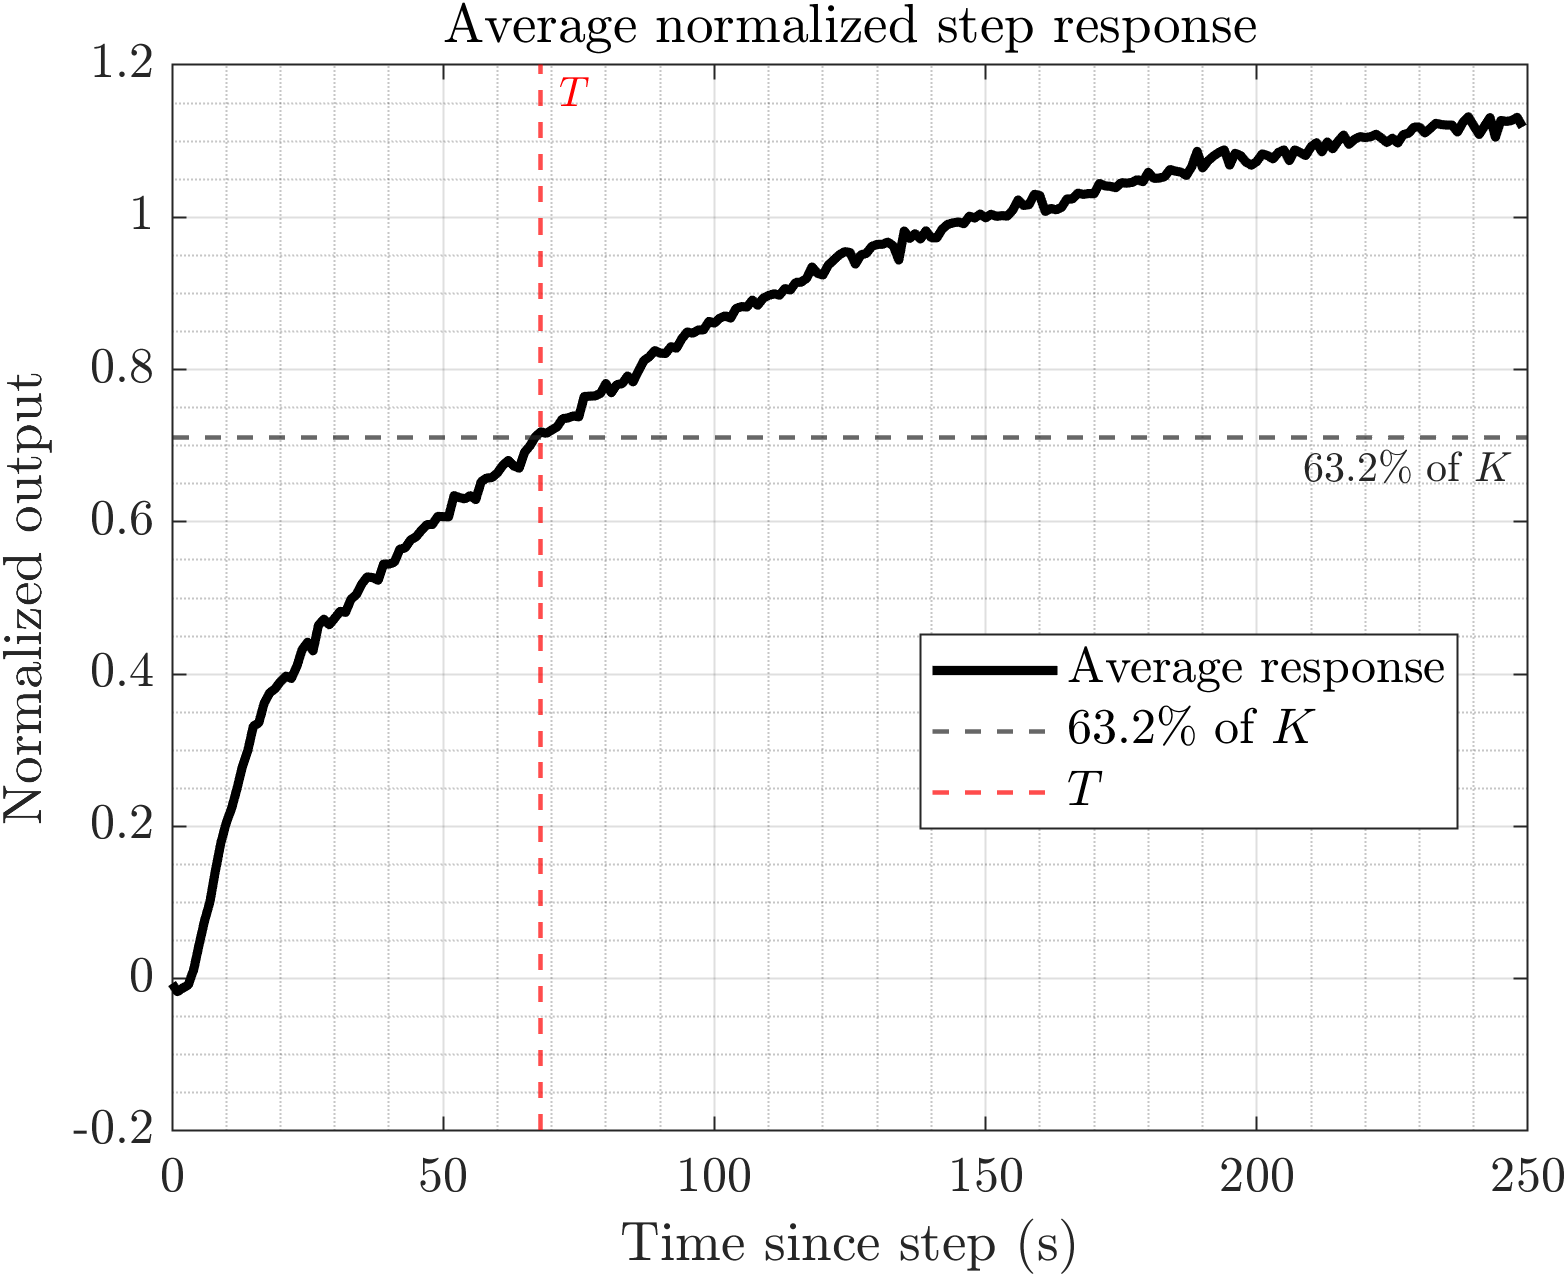
\includegraphics[width=0.8\textwidth]{images/fig_average_step_response.png}
    \caption{Average normalized step response used for linear model identification.}
    \label{fig:avg_step}
\end{figure}

Based on the averaged step response, a first-order linear model was identified. The steady-state gain $K$ was estimated from the final value of the response, while the time constant $\tau$ was determined using the $63.2\%$ criterion.

For the identified process, the estimated parameters were
\begin{equation}
K \approx 1.17, \qquad \tau \approx 68~\mathrm{samples}.
\label{eq:strejc_identified_parameters}
\end{equation}

With a sampling period of $T_s = 1~\mathrm{s}$, the continuous-time model was converted into a discrete-time state-space representation. For a first-order system, the discrete-time coefficients are given by
\begin{equation}
A = e^{-T_s/\tau}, \qquad
B = K \left(1 - e^{-T_s/\tau}\right), \qquad
C = 1, \qquad
D = 0.
\end{equation}

Substituting the identified parameters into the discrete-time model introduced in equation~\eqref{eq:strejc_state} and \eqref{eq:strejc_state2} yields the following representation:
\begin{equation}
x_{k+1} = 0.985\,x_k + 0.016\,u_k,
\qquad
y_k = x_k.
\end{equation}

The identified linear model was subsequently used as the prediction model in the baseline MPC design, following common practice in industrial control applications \cite{rawlings_mpc}.

To evaluate the model's predictive capability, an open-loop simulation was performed on the test dataset. In this setting, the measured input signal was applied directly to the model, while the output was not corrected using measurements. The resulting trajectory, therefore, represents a pure model prediction driven only by the input signal and the initial condition.

The model parameters were identified using the complete dataset. For validation, the data were split, and the second part of the experiment, starting at $t = 2250~\mathrm{s}$, was used for open-loop testing.

The predicted output $\hat{y}_k$ was compared with the measured outlet temperature $y_k = T_4$, and the prediction error was first quantified using the mean square error (MSE),
\begin{equation}
\mathrm{MSE} =
\frac{1}{N_{\mathrm{s}}} \sum_{k=1}^{N_{\mathrm{s}}}
\left( y_k - \hat{y}_k \right)^2,
\label{eq:mse}
\end{equation}
where $N_{\mathrm{s}}$ denotes the number of samples in the testing dataset.

The root mean square error (RMSE) was then computed as
\begin{equation}
\mathrm{RMSE} =
\sqrt{\mathrm{MSE}}
=
\sqrt{\frac{1}{N_{\mathrm{s}}} \sum_{k=1}^{N_{\mathrm{s}}}
\left( y_k - \hat{y}_k \right)^2}.
\label{eq:rmse}
\end{equation}
The RMSE was computed in physical units after reversing the data scaling.

For the identified linear model, the overall open-loop RMSE$_{\mathrm{OL}}$ obtained on the test data was
\begin{equation}
\mathrm{RMSE}_{\mathrm{OL}} = 1.6962~^{\circ}\mathrm{C}.
\label{eq:rmseOL}
\end{equation}


This value is a direct measure of model accuracy, reflecting the model's ability to predict the process output in open-loop conditions. The results indicate that the model captures the main thermal dynamics of the heat exchanger. However, prediction errors accumulate over time due to nonlinearities and unmodeled disturbances \cite{ljung_sysid}. The identified linear model is valid primarily around the operating region and may lose accuracy for larger deviations from this region due to nonlinear effects.
Although the model is sufficient for basic control design, this limitation motivates the use of more expressive data-driven models, such as the Koopman-based approach introduced in the following sections.

\subsection{Koopman-based Identification of a Heat Exchanger}
\label{sec:koopman_identification}

This subsection summarizes how the Koopman prediction model used later for control was obtained. While Section~\ref{sec:Koopman_operator} presents the general Koopman framework, here we focus on the specific model structure, training setup, and how the final state-space matrices were extracted.

The identification was carried out using the \texttt{Neuromancer} framework~\cite{neuromancer2022}, which enables efficient training of data-driven dynamical models. Before training, the measured output and input signals were standardized using precomputed \texttt{StandardScaler} objects, defined by the mean and standard deviation of the training data. This is a standard practice used to improve numerical conditioning during neural network training \cite{goodfellow2016deep}. The scaling parameters used in this work were
\begin{equation}
\mu_y = 59.0676, \qquad \sigma_y = 6.9122,
\label{eq:output_scaling_parameters}
\end{equation}
\begin{equation}
\mu_u = 65.8447, \qquad \sigma_u = 22.9062.
\label{eq:input_scaling_parameters}
\end{equation}



We used an encoder--decoder architecture with control inputs. The measured outlet temperature $y_k$ was lifted to a latent state $z_k \in \mathbb{R}^{n_z}$ with $n_z = 10$ using a fully connected multi-layer perceptron with three hidden layers $[60,\,60,\,60]$ and ReLU activations. The input $u_k$ was mapped to the same latent dimension by a linear layer without bias.

The latent dynamics were represented by the controlled Koopman model given in Equation~\eqref{eq:koopman_state}, where $A_{\mathcal K}$ corresponds to a trainable linear layer and $B_{\mathcal K}$ represents the influence of the control input in the lifted space. The output was reconstructed by the linear decoder given in Equation~\eqref{eq:koopman_output}. The Koopman matrices used later in MPC correspond directly to the learned network weights. The total number of trainable parameters was $8170$.

Training was performed on data segments of $n_{\mathrm{steps}} = 50$ and mini-batches of size $b_s = 100$. The Adam optimizer was employed with a learning rate of $10^{-3}$ and a fixed random seed, following best practices in neural network training \cite{kingma2015adam}. The maximum number of epochs was set to $900$, with early stopping based on the development loss, a patience of $200$ epochs, and a warmup period of $100$ epochs. The training duration was approximately $35$ minutes on a single GPU.

The measured dataset was split into training and testing parts for model validation. In contrast, the parameters of the linear model were obtained from averaged step responses computed from the measured data. The raw measured input and output signals used for identification are shown in Figure~\ref{fig:raw_measurements}.

Training minimized a weighted sum of loss terms that penalize prediction errors and enforce consistency of the lifted representation. In contrast to the general formulation presented in Section~\ref{sec:Koopman_operator}, the practical implementation used the weighting coefficients
\begin{equation}
\alpha_y = 10, \qquad
\alpha_{\mathrm{1step}} = 1, \qquad
\alpha_{\mathrm{rec}} = 20, \qquad
\alpha_x = 1.
\label{eq:koopman_loss_weights}
\end{equation}
Here, $\alpha_y$ weights the multi-step output prediction loss, $\alpha_{\mathrm{1step}}$ weights the one-step prediction loss, $\alpha_{\mathrm{rec}}$ weights the reconstruction loss, and $\alpha_x$ weights the latent consistency loss.

These loss terms correspond to the objectives of accurate multi-step prediction, local one-step accuracy, encoder--decoder consistency, and linear evolution in the lifted space. The corresponding mean squared errors were approximately
\begin{equation}
\mathrm{MSE}_{\mathrm{train}} \approx 0.068, \qquad
\mathrm{MSE}_{\mathrm{val}} \approx 0.060.
\label{eq:koopman_train_val_mse}
\end{equation}

In this implementation, no explicit stability constraint on the Koopman operator was imposed, i.e., a standard linear layer was used instead of a constrained singular value decomposition (SVD) parameterization. The model is linear in the lifted space but represents nonlinear input–output behavior.

The identified Koopman model was then evaluated in open loop on the available test trajectory. The resulting open-loop error was
\begin{equation}
\mathrm{RMSE}_{\mathrm{OL}}^{\mathrm{Koop}} = 1.6681~^{\circ}\mathrm{C}.
\label{eq:koopman_rmseOL}
\end{equation}

The results indicate that the Koopman model achieves a slightly lower prediction error compared to the first-order model. The difference is relatively small, suggesting that both models capture the dominant system dynamics, while the Koopman model provides a marginal improvement by representing nonlinear effects.

The identified matrices \(A_{\mathcal K}\), \(B_{\mathcal K}\), and \(C_{\mathcal K}\) were determined from the trained neural Koopman model as the linear operators describing, respectively, the state evolution in the lifted space, the effect of the control input, and the mapping from the lifted state back to the measured output. The direct feedthrough term was assumed to be zero, i.e., \(D_{\mathcal K}=0\). These matrices were then used in the subsequent Koopman-based MPC formulation and in the experimental evaluation on the heat exchanger system.

For a visual comparison, Figure~\ref{fig:open_loop_compare} shows the measured test output alongside the open-loop predictions from both identified models. The linear model follows the dominant trend of the measured response well, while the Koopman model provides comparable predictive performance. The figure confirms that both models are suitable for subsequent controller design, although both accumulate prediction error over longer horizons.

\begin{figure}[htbp]
    \centering
    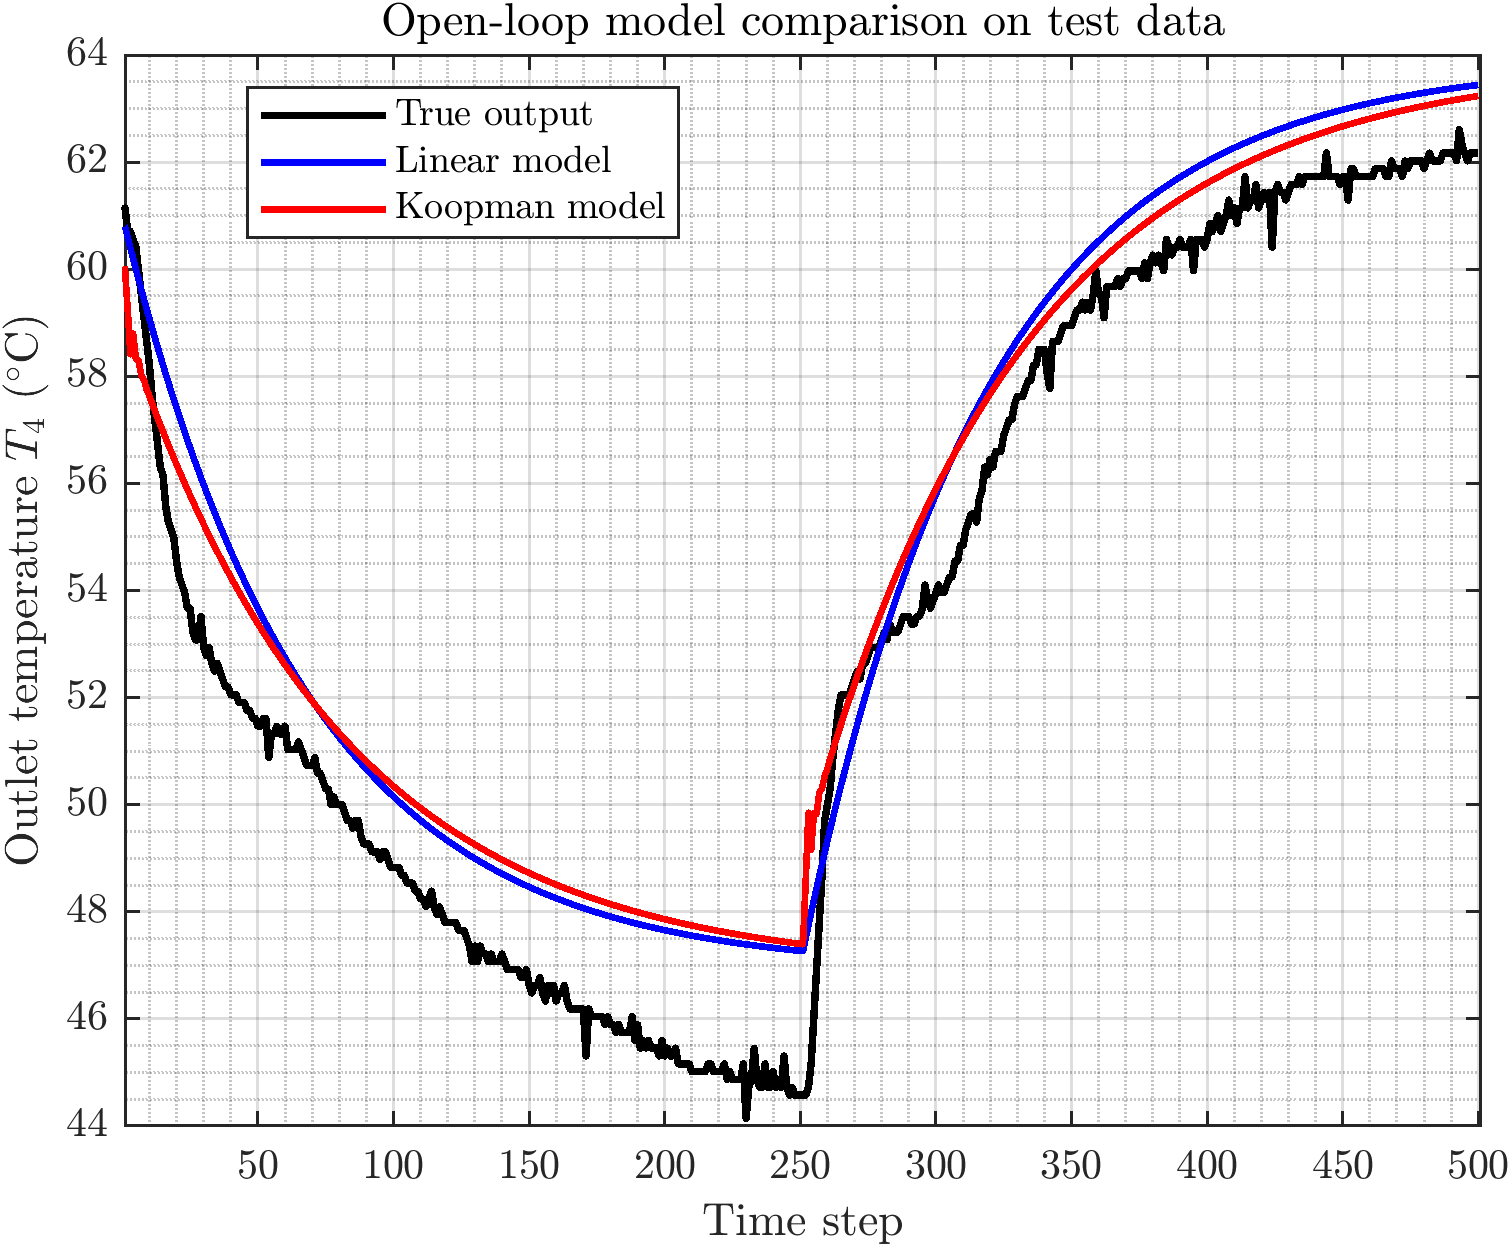
\includegraphics[width=0.9\textwidth]{images/open_loop_model_comparison.png}
    \caption{Open-loop comparison of the measured outlet temperature $T_4$ and the predicted outputs of the linear step-response model and the Koopman model on the test dataset.}
    \label{fig:open_loop_compare}
\end{figure}


\section{MPC Controller Design}
\label{sec:mpc_design}

Based on the identified process models described in the previous sections, MPC was designed for both the linear model and the data-driven Koopman model. In both cases, the control
objective is to regulate the outlet temperature of the heat exchanger
around a fixed operating point. The reference was set to zero in the
normalized coordinates, corresponding to the empirical mean temperature
used during model identification.


\subsection{Koopman-based MPC}

For the Koopman-based controller, the prediction horizon was set to $N = 20$ samples. The prediction model is given by the Koopman system matrices identified in Equations~\eqref{eq:koopman_state} and~\eqref{eq:koopman_output}. The lifted state vector has dimension $n_z = 10$, corresponding to the learned latent representation of the measured temperature and input.


Since only the outlet temperature $T_4$ is measured, a KF is used to estimate the lifted Koopman state. The filter was implemented using constant covariance matrices
\begin{equation}
Q_{\mathrm{KF}} = 0.5\,I, \qquad R_{\mathrm{KF}} = 0.1,
\label{eq:kf_covariances}
\end{equation}
which were selected systematically to achieve satisfactory estimation performance.


To evaluate closed-loop performance over the entire experiment of length $N_{\mathrm{CL}}$ samples, the cumulative cost was computed as
\begin{equation}
    J_{\mathrm{CL}} =
    \sum_{t=0}^{N_{\mathrm{CL}}-1}
    \left(
        \|y_t\|_{Q}^{2} + \|u_t\|_{R}^{2}
    \right),
    \label{eq:closed_loop_cost}
\end{equation}
with weights $Q = 10$ and $R = 1$. The weights were selected empirically to balance tracking performance and control effort.



Input and output constraints were enforced directly in the optimization
problem. The pump speed was limited to the interval
\[
20~\% \leq u_k \leq 100~\%,
\]
and the outlet temperature was constrained to
\[
0~^\circ\mathrm{C} \leq y_k \leq 70~^\circ\mathrm{C}.
\]

The resulting quadratic program was solved online using the \texttt{quadprog} solver via the YALMIP~\cite{lofberg2004yalmip} optimization framework.

\subsection{Linear-based MPC}


The linear-based MPC uses the same controller structure as the
Koopman-based MPC. In particular, the cost function weights
$(Q = 10,\, R = 1)$, the actuator and output constraints, and the
KF parameters $(Q_{\mathrm{KF}}, R_{\mathrm{KF}})$ as well as the prediction horizon $N$ were chosen
identically. 

By keeping the MPC formulation and tuning parameters consistent across
both controllers, any observed differences in control performance can be
related to primarily to the quality of the underlying prediction model
rather than to differences in controller design.

\section{Simulation Results}
\label{sec:simulation_results}

Closed-loop simulations were performed to compare the Koopman-based MPC and the MPC based on a linear model identified from the step response under the same constraints and tuning described in Section~\ref{sec:mpc_design}. The simulations were carried out over a horizon of $150$ time steps, and both controllers were tested from several initial outlet temperatures
\[
T_0 \in \{45,50,55,58,60,62,66,68\}\,^{\circ}\mathrm{C}.
\]

A nonlinear data-driven baseline model was used as the simulation plant. This model was identified using the NeuroMANCER framework in Python and represented outlet temperature dynamics in a lifted latent space. The baseline model combines neural-network-based lifting and reconstruction with linear latent-state evolution, enabling a more accurate representation of nonlinear input–output behavior \cite{yeung2019learning, otto2019linearly}.

The baseline model uses an encoder--decoder structure. The measured outlet temperature is mapped by an encoder neural network into a latent state vector $z^{\mathrm{b}}$. This latent vector contains 24 variables, which are used to represent the state of the process. The latent-state evolution is modeled by a linear operator, and the effect of the control input is included through a separate input mapping. A decoder neural network maps the latent state back to the predicted physical output.

The latent dynamics of the baseline model are described by the discrete-time model
\begin{equation}
    z^{\mathrm{b}}_{k+1} = A^{\mathrm{b}}_{\mathcal{K}} z^{\mathrm{b}}_k + B^{\mathrm{b}}_{\mathcal{K}} u_k.
\label{eq:baseline_latent_dynamics}
\end{equation}
where $z^{\mathrm{b}}_k$ denotes the lifted latent state of the baseline model and $u_k$ is the control input. The physical output is reconstructed as
\begin{equation}
\hat{y}^{\mathrm{b}}_k = f^{\mathrm{b}}_{\mathrm{dec}}\left(z^{\mathrm{b}}_k\right),
\label{eq:baseline_decoder}
\end{equation}
where $f^{\mathrm{b}}_{\mathrm{dec}}(\cdot)$ denotes the decoder network of the baseline model.


It is important to note that these closed-loop simulations are primarily intended to verify that both predictive controllers can drive the simulated plant to the desired steady-state region in a stable and consistent manner. The simulation study serves mainly as a comparative validation of controller behavior on a common reference model, rather than an exact replication of the real experimental device.

A representative example of the simulation is shown in Figure~\ref{fig:cl_response45} for the initial temperature $T_0 = 45,^{\circ}\mathrm{C}$, i.e., for an initial condition significantly below the steady-state operating region. In this case, both controllers first apply a strong control action at the actuator limit and then gradually reduce the input as the output approaches steady state. The responses show that both MPC formulations can regulate the system from a large initial deviation toward the steady-state. 

\begin{figure}[!t]
    \centering
    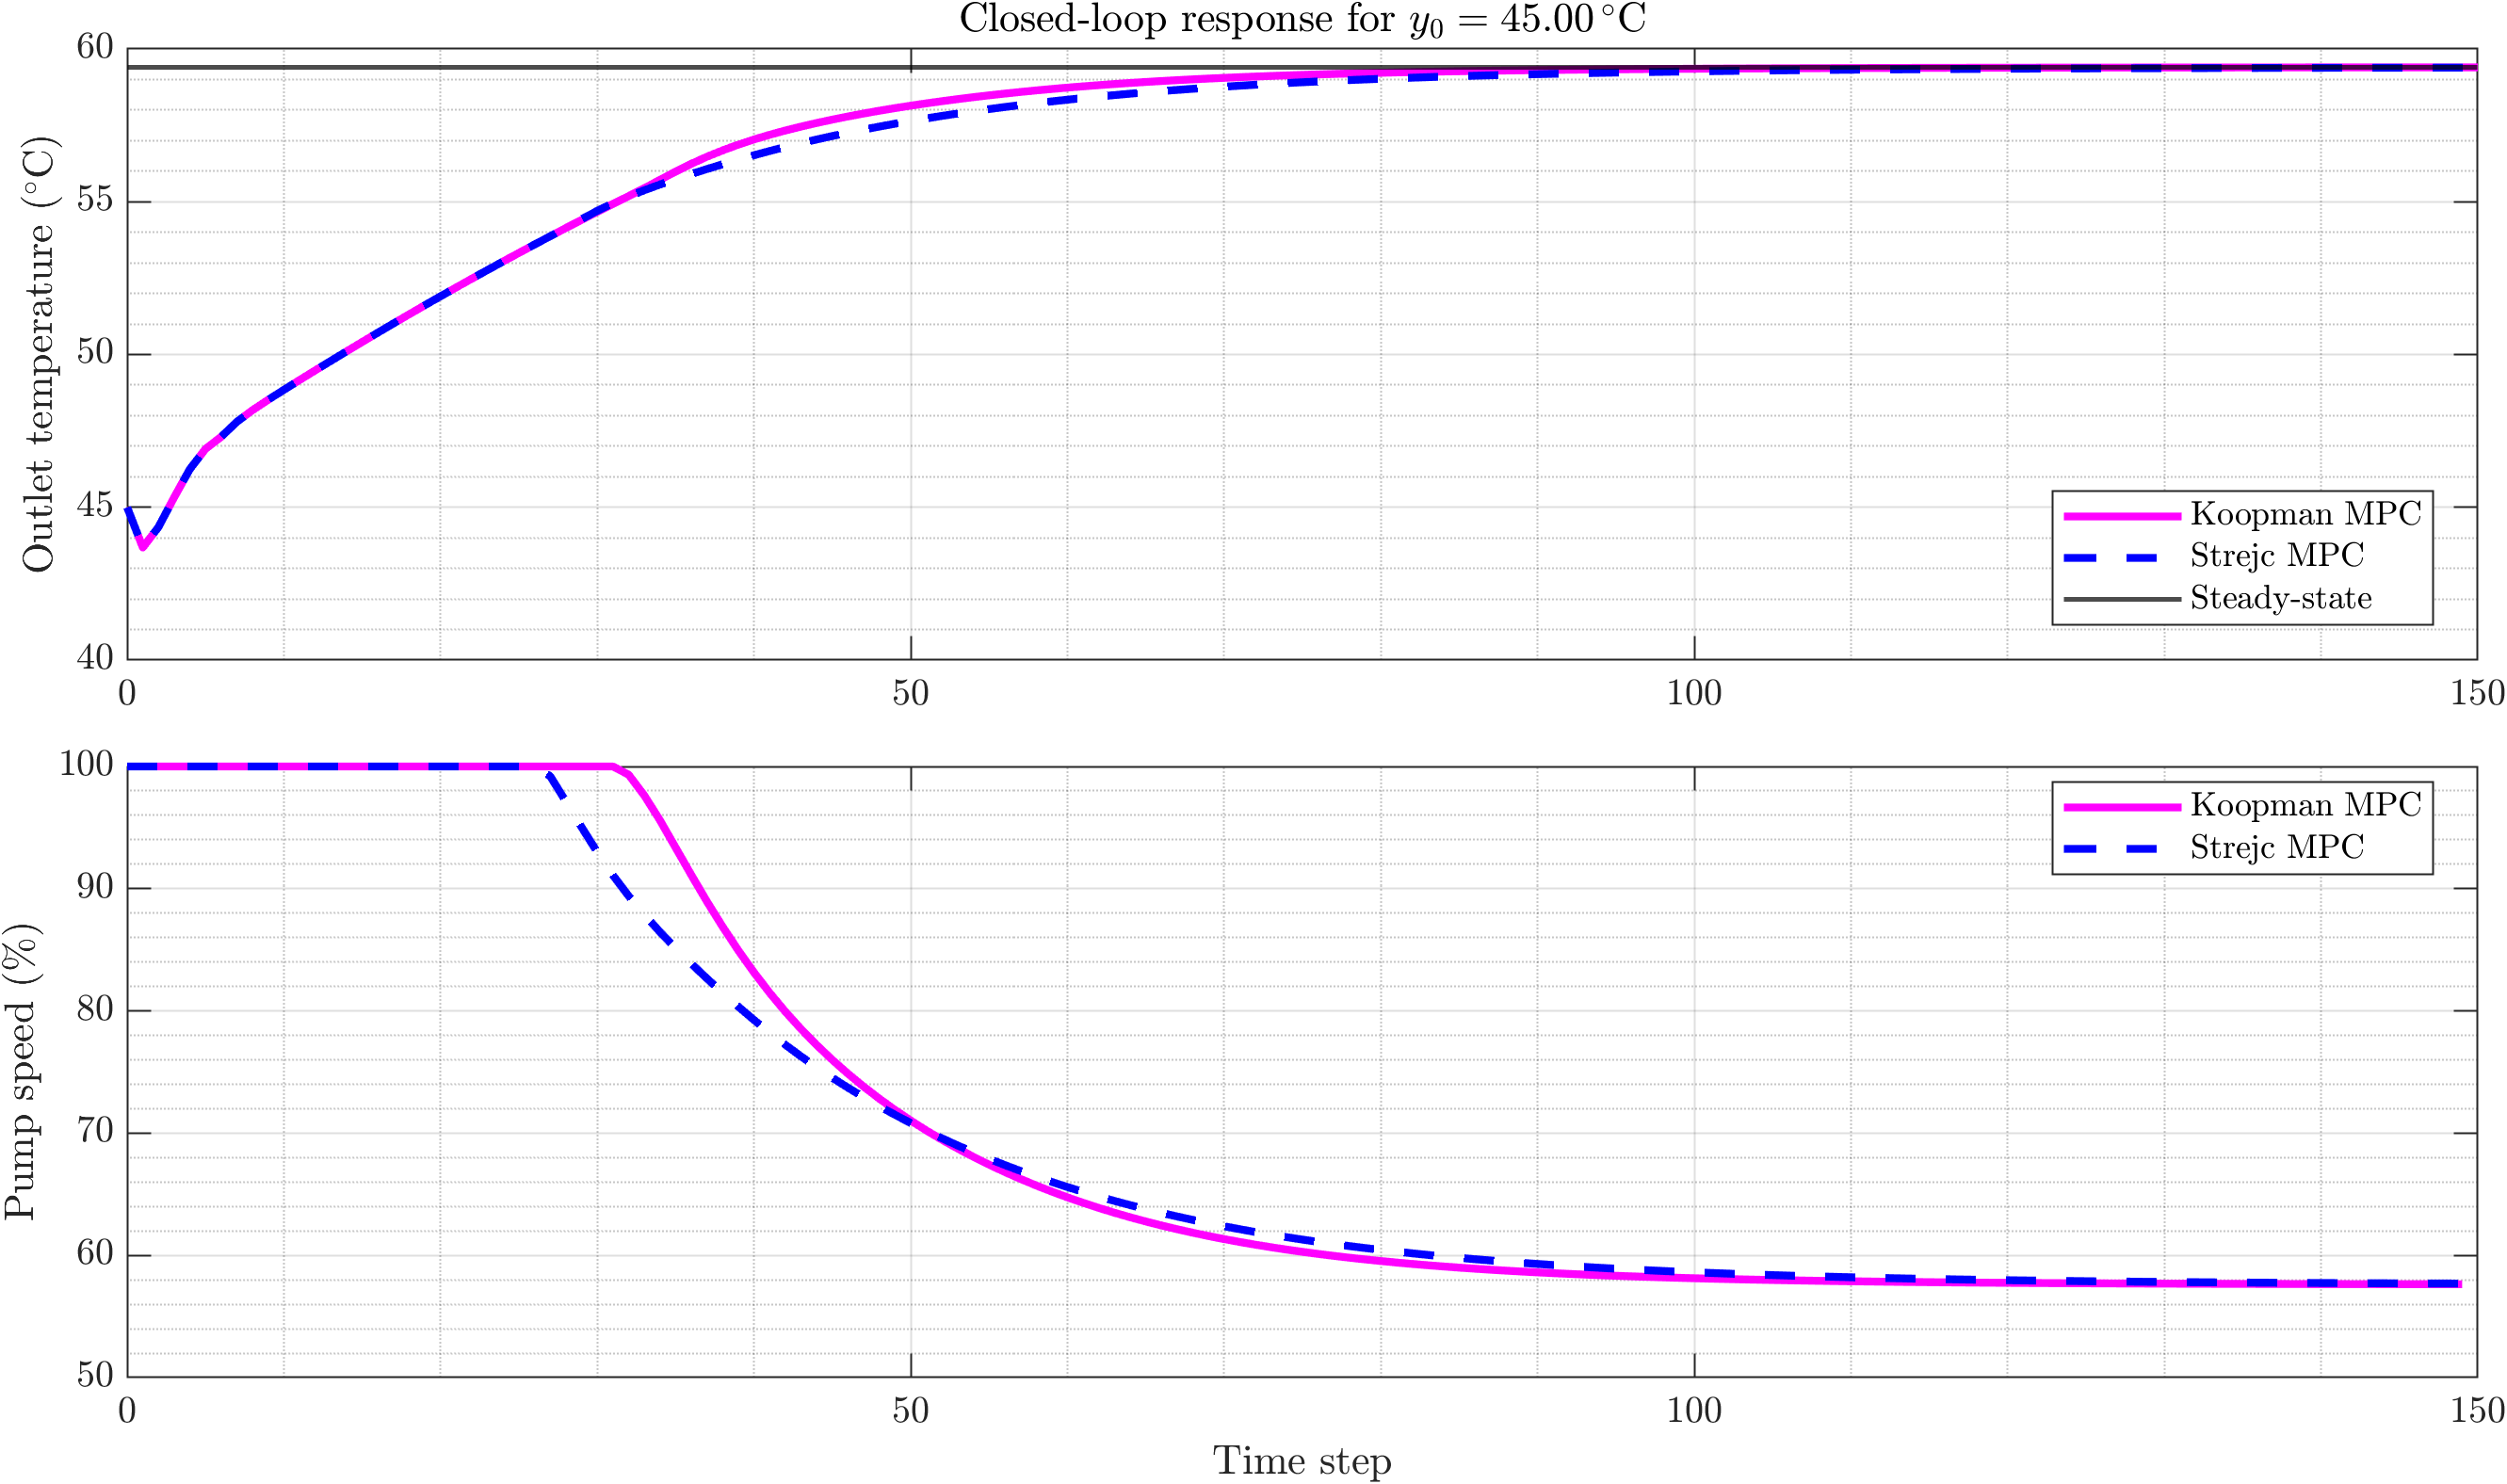
\includegraphics[width=0.95\textwidth]{images/IC_01_y0_45_00.png}
    \caption{Closed-loop response and control input comparison for Koopman MPC and MPC based on the linear model identified from step response for the initial condition $T_0 = 45\,^{\circ}\mathrm{C}$. This case illustrates that both controllers regulate the simulated plant to the steady-state operating region, also from a large initial deviation.}
    \label{fig:cl_response45}
\end{figure}

To evaluate closed-loop performance, three metrics were considered: root mean square error (RMSE), integral of absolute error (IAE), and the closed-loop quadratic objective value. The IAE is defined as
\begin{equation}
\mathrm{IAE} = \sum_{k=1}^{N_{\mathrm{sim}}} \left| y(k) - y_{\mathrm{ss}} \right|,
\label{eq:iae}
\end{equation}
where $y(k)$ denotes the outlet temperature at time step $k$, $y_{\mathrm{ss}}$ is the steady-state operating point, and $N_{\mathrm{sim}}$ is the simulation length.

Each metric looks at a different piece of how the closed-loop system behaves. RMSE highlights big swings away from the steady-state—since the errors are squared, the metric puts more weight on large deviations. This helps when trying to determine how severe the prevailing transient errors are. IAE, on the other hand, tracks the total absolute error over the whole simulation. It is less influenced by isolated spikes, so it's useful for understanding not just how much, but how long the system strays from its target. Then, the closed-loop objective, $J_{\mathrm{CL}}$, is rooted in the quadratic criterion from the MPC setup. That combines both how far the system deviates and how much control effort it takes, giving a clear sense of the overall cost relative to the controller's target.

For the initial condition $T_0 = 45\,^{\circ}\mathrm{C}$, the Koopman MPC achieved $\mathrm{RMSE}=4.58\,^{\circ}\mathrm{C}$, $\mathrm{IAE}=358.28$, and $J_{\mathrm{CL}}=563.53$, whereas the MPC based on the linear model identified from the step response achieved $\mathrm{RMSE}=4.62\,^{\circ}\mathrm{C}$, $\mathrm{IAE}=380.57$, and $J_{\mathrm{CL}}=562.36$. Although the quadratic objective values are almost identical in this case, the Koopman MPC yields slightly smaller tracking errors in both RMSE and IAE.

When averaged over all tested initial conditions, the mean RMSE is $1.59\,^{\circ}\mathrm{C}$ for the Koopman MPC and $1.65\,^{\circ}\mathrm{C}$ for the linear-model-based MPC. The mean IAE values are $115.77$ and $130.41$, respectively. The mean closed-loop objective values are $131.37$ and $131.79$, which are nearly identical.

Table~\ref{tab:performance_metrics} summarizes the results for all tested initial temperatures. For initial conditions close to the operating point, both controllers achieve very small tracking errors. As the initial temperature moves further from the reference, both RMSE and IAE increase, as expected due to larger transient deviations and stronger control action requirements.

\begin{table}[!t]
    \centering
    \caption{Performance metrics for Koopman MPC and MPC based on a linear model identified from step response, evaluated for different initial temperatures.}
    \label{tab:performance_metrics}
    \begin{tabular}{c|ccc|ccc}
    \hline
    \multirow{2}{*}{$T_0$ [$^\circ$C]} &
    \multicolumn{3}{c|}{Koopman MPC} &
    \multicolumn{3}{c}{Linear step-response MPC} \\
     & RMSE [$^\circ$C] & IAE & $J_{\mathrm{CL}}$ &
     RMSE [$^\circ$C] & IAE & $J_{\mathrm{CL}}$ \\
    \hline
    45 & 4.58 & 358.28 & 563.53 & 4.62 & 380.57 & 562.36 \\
    50 & 2.93 & 209.77 & 259.79 & 2.98 & 231.62 & 257.93 \\
    55 & 1.49 & 97.24  & 82.05  & 1.54 & 114.97 & 79.22  \\
    58 & 0.64 & 40.95  & 15.78  & 0.67 & 48.89  & 15.32  \\
    60 & 0.32 & 20.40  & 3.80   & 0.33 & 24.08  & 3.76   \\
    62 & 0.23 & 8.78   & 1.71   & 0.24 & 10.45  & 1.90   \\
    66 & 0.99 & 70.94  & 36.89  & 1.10 & 86.72  & 39.44  \\
    68 & 1.53 & 119.82 & 87.43  & 1.70 & 145.97 & 94.37  \\
    \hline
    \textbf{Mean} &
    \textbf{1.59} & \textbf{115.77} & \textbf{131.37} &
    \textbf{1.65} & \textbf{130.41} & \textbf{131.79} \\
    \hline
    \end{tabular}
\end{table}

The same trend can be observed for both controllers. When the initial temperature is close to the operating point, the transient deviation is small and the RMSE and IAE values remain low. For larger initial deviations, the response takes longer to reach the steady-state region, which leads to higher accumulated errors. A similar trend is also reflected in the closed-loop objective value.

The results do not indicate a strong dominance of one controller over the other across all operating conditions. However, the Koopman MPC achieves slightly lower RMSE across all tested initial temperatures and lower IAE in every case. This suggests that the Koopman-based prediction model provides a slightly better overall tracking quality on the considered simulation plant, even though the differences remain relatively small.




All three performance metrics are also visualized in Figure~\ref{fig:sim_metrics_summary}.

\begin{figure}[H]
    \centering
    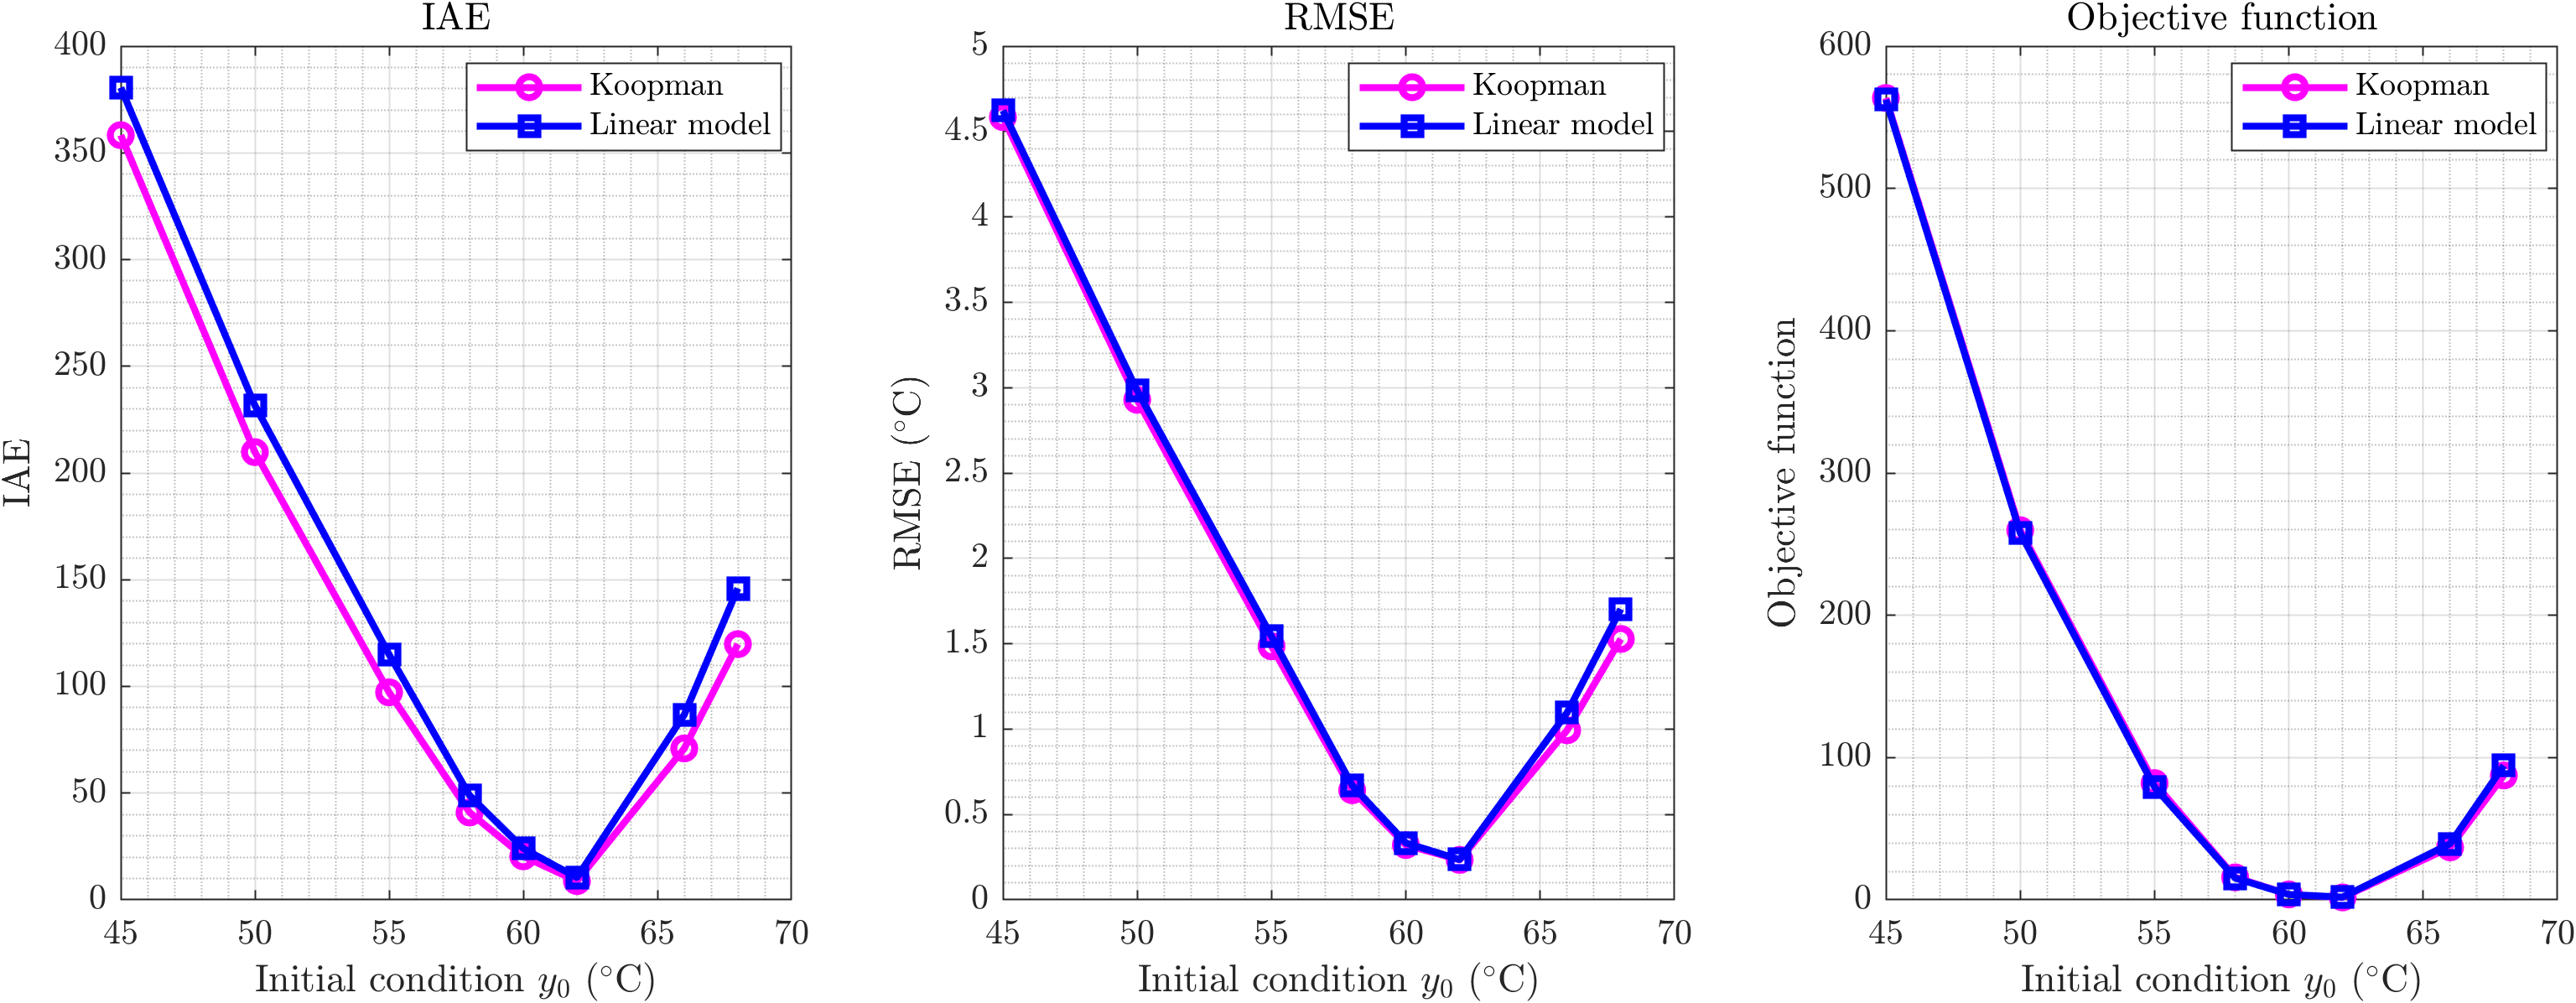
\includegraphics[width=\textwidth]{images/Summary_metrics.png}
    \caption{Closed-loop performance metrics versus initial temperature $T_0$ for Koopman MPC and MPC based on the linear model identified from step response: IAE, RMSE, and the closed-loop objective value $J_{\mathrm{CL}}$.}
    \label{fig:sim_metrics_summary}
\end{figure}

From these results we can say that they depend on the plant's operating range. The heat exchanger's slow thermal dynamics mean a simple linear step-response model already captures most of the system's behavior. That's why both MPC controllers, classic and Koopman, end up producing nearly the same closed-loop performance. The controllers also use the same MPC setup—same constraints, horizon, and weights. The objective function penalizes tracking errors and control effort, so even if the Koopman controller tracks a bit better, it hardly moves $J_{\mathrm{CL}}$ downward.


\section{Experimental Results}
\label{sec:experimental_results}

Experimental validation was performed on the Armfield PCT23 heat exchanger described in Section~\ref{sec:practical_introduction}.
The goal was to verify the closed-loop behavior observed in simulations on the real device and to compare the Koopman-based MPC with the MPC based on a first-order linear model under identical experimental conditions.

The experiments were initialized at different outlet temperatures.
Before each MPC run, the desired starting temperature was achieved using a PI controller acting on the pump speed.

Regulation was performed to zero in normalized coordinates.
The corresponding reference temperature $x_{\text{target}} = 63.808^{\circ}\mathrm{C}$ was computed from the measured steady-state mean obtained during the experimental day.
This value is consistent with the input mean $u_{\text{mean}}$ used during identification, but it does not correspond to the mean of the identification dataset itself.
The prediction horizon, cost function weights, constraints, and Kalman filter parameters were kept identical for both controllers, so that only the difference between the prediction models is compared.

During the experiments, the outlet temperature $T_4$ was used as the feedback signal.
The heater loop and the pump in the secondary circuit were kept unchanged.
The only manipulated variable was the pump speed controlled by the MPC.

\begin{figure}[!ht]
\centering
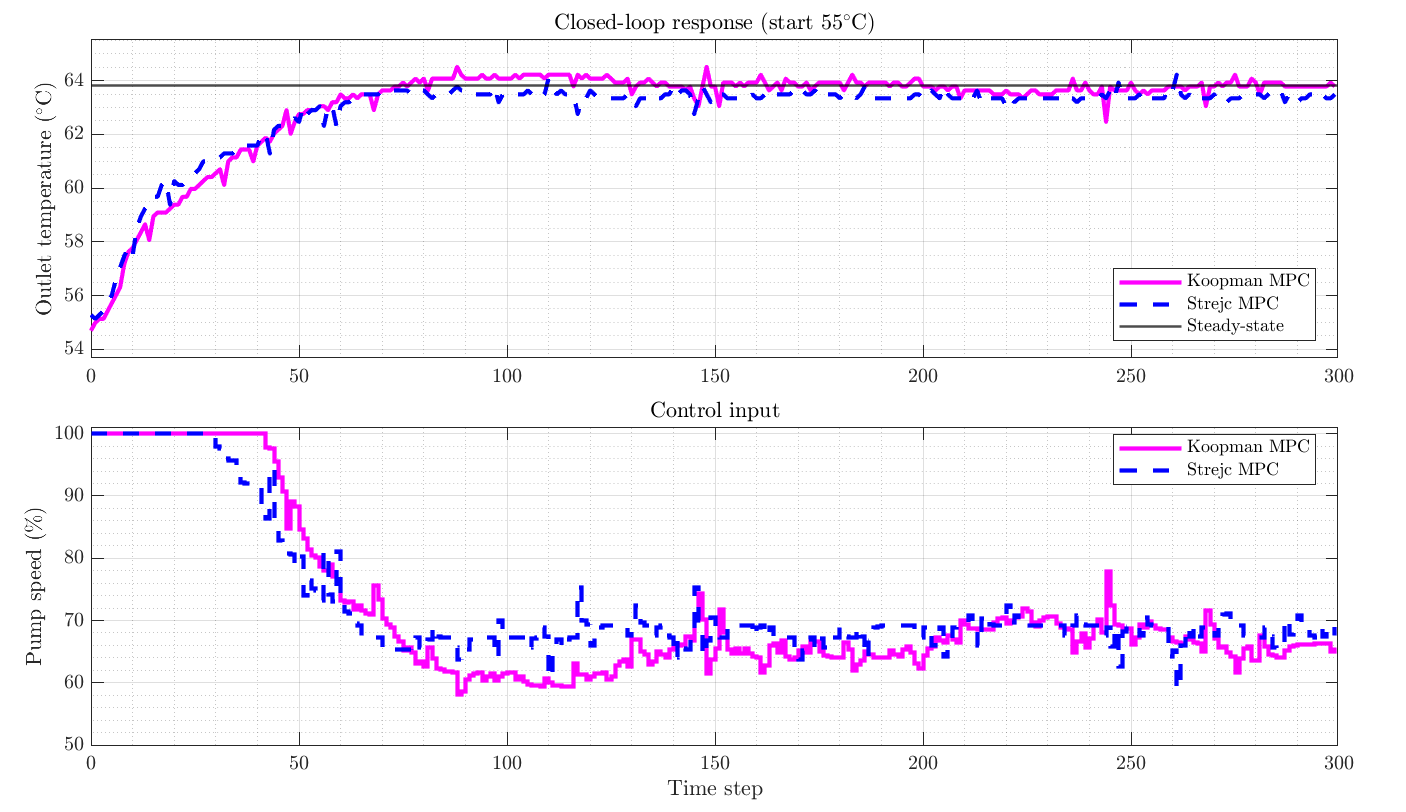
\includegraphics[width=\textwidth]{images/compare_cl_T0_55.png}
\caption{Experimental closed-loop response and control input for the initial temperature $T_0 = 55,^{\circ}\mathrm{C}$.}
\label{fig:cl_exp_T0_55}
\end{figure}

Figure~\ref{fig:cl_exp_T0_55} shows the experimental closed-loop response for the case starting from
$T_0 = 55,^{\circ}\mathrm{C}$.
Both controllers regulate the outlet temperature towards the operating point and reach a stable steady-state region.

At the beginning of the experiment, both controllers apply a strong control action close to the actuator limits.
The Koopman MPC remains at the upper input constraint for slightly longer and exhibits more aggressive behavior, leading to a small temperature overshoot.
The linear MPC reduces the input earlier and follows a smoother trajectory towards the steady state.

In terms of performance metrics, both controllers achieve comparable results.
For $T_0 = 55,^{\circ}\mathrm{C}$, the RMSE is $2.004,^{\circ}\mathrm{C}$ for the Koopman MPC and $1.872,^{\circ}\mathrm{C}$ for the linear MPC.
The IAE values are $272.46$ and $296.91$, respectively.
The objective function value is lower for linear MPC, indicating smoother control actions and smaller input variations.

The differences can be related to the behavior of the real system.
The heat exchanger exhibits nonlinearities and disturbances that neither model fully captures.
The Koopman MPC tends to respond more strongly when the temperature is below the expected value, leading to larger initial control actions and occasional overshoot.
The linear MPC behaves more conservatively, leading to slightly lower RMSE but slower input adjustment.

Overall, both controllers provide consistent and stable regulation of the system.
The main differences are visible in the transient phase, particularly in the aggressiveness of the control input and the speed of convergence.

\begin{figure}[!ht]
\centering
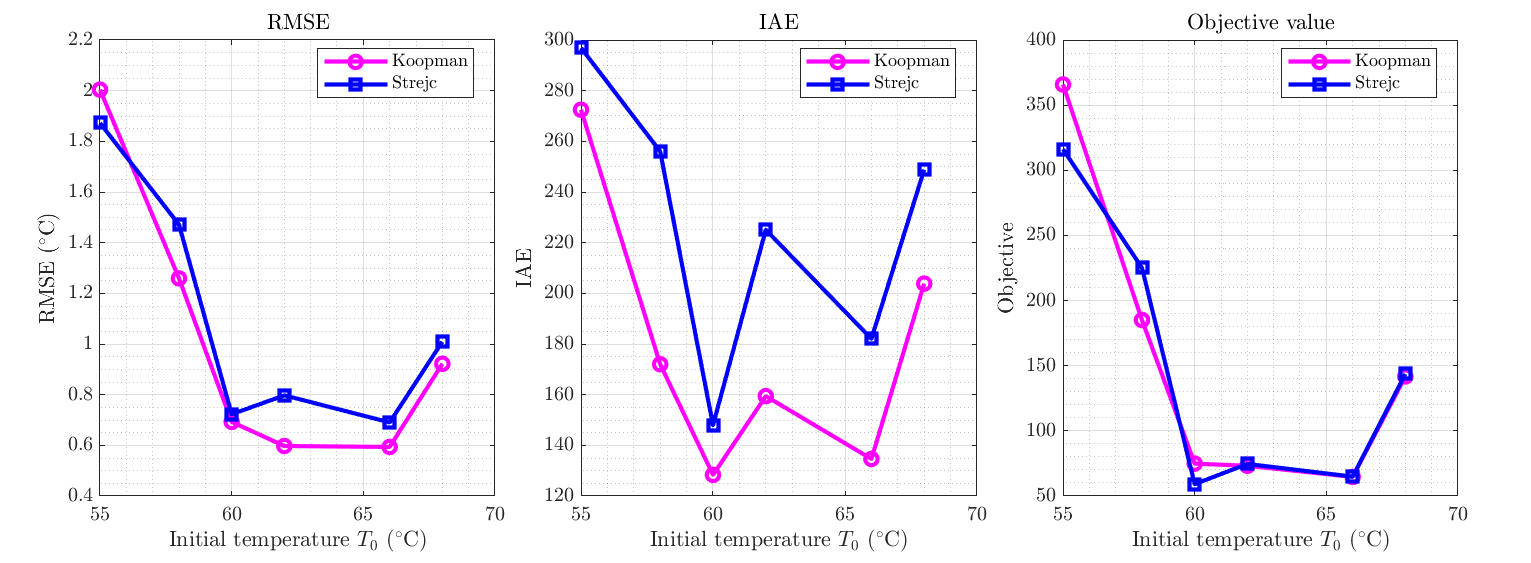
\includegraphics[width=\textwidth]{images/metrics_vs_T0_from55.png}
\caption{Experimental performance metrics (RMSE, IAE, and objective value) evaluated for different initial outlet temperatures $T_0$.}
\label{fig:exp_metrics}
\end{figure}

Figure~\ref{fig:exp_metrics} summarizes the experimental performance metrics for all tested initial conditions.
The RMSE decreases as the initial temperature approaches the operating point and reaches its minimum in the interval
$T_0 = 60$--$66,^{\circ}\mathrm{C}$ for both controllers.

The IAE shows a similar dependence on the initial condition.
The lowest IAE values are obtained near the operating point and increase as the initial temperature moves farther away.
Table~\ref{tab:performance_metrics_exp} summarizes the performance metrics for all tested initial temperatures.

\begin{table}[!t]
\centering
\caption{Performance metrics for Koopman MPC and linear MPC obtained from experiments for different initial temperatures.}
\label{tab:performance_metrics_exp}
\begin{tabular}{c|ccc|ccc}
\hline
\multirow{2}{*}{$T_0$ [$^\circ$C]} &
\multicolumn{3}{c|}{Koopman MPC} &
\multicolumn{3}{c}{Linear MPC} \\
& RMSE [$^\circ$C] & IAE & $J_{\mathrm{CL}}$ &
RMSE [$^\circ$C] & IAE & $J_{\mathrm{CL}}$ \\
\hline
55 & 2.004  & 272.46 & 365.86 & 1.872 & 296.91 & 316.18 \\
58 & 1.259  & 172.00 & 185.07 & 1.471 & 256.00 & 225.12 \\
60 & 0.693  & 128.34 & 74.84  & 0.723 & 147.94 & 59.08  \\
\rowcolor{gray!15}
62 & 0.597  & 159.42 & 73.19  & 0.797 & 225.07 & 74.61  \\
66 & 0.594  & 134.62 & 64.63  & 0.690 & 182.05 & 64.86  \\
68 & 0.922  & 203.83 & 141.72 & 1.009 & 248.83 & 143.66 \\
\hline
\textbf{Mean} &
\textbf{1.011} & \textbf{178.45} & \textbf{150.88} &
\textbf{1.094} & \textbf{226.13} & \textbf{147.25} \\
\textbf{Sum}  &
\textbf{6.068} & \textbf{1070.67} & \textbf{905.31} &
\textbf{6.563} & \textbf{1356.80} & \textbf{883.50} \\
\hline
\end{tabular}
\end{table}



The experimental results can be explained by the different properties of the two prediction models and by the behavior of the real heat exchanger. The real system contains nonlinear heat-transfer effects, measurement noise, actuator limitations, and small disturbances from the hydraulic and thermal circuits. These effects are not captured perfectly by either prediction model, which explains why the experimental responses differ more than the simulation responses.

Koopman MPC usually achieves a lower IAE because its lifted prediction model captures the process's transient nonlinear behavior more accurately. This helps the controller lower the tracking error throughout the experiment. At the same time, this property makes the Koopman controller react more quickly to any deviation from the operating point. So, if the measured temperature drops below the steady-state target, the controller pushes a stronger input and tends to stay near the actuator limit longer. The error drops quickly, but that same aggressiveness can lead to overshoot and sometimes a slightly higher RMSE, like in the case where $T_0 = 55\,^{\circ}\mathrm{C}$.

Linear MPC, on the other hand, uses a first-order model based on averaged step responses, so it mainly tracks the dominant slow thermal dynamics of the heat exchanger. This makes the control response smoother and more cautious, especially during the early transient phase. Because the closed-loop cost penalizes input effort, the linear MPC can sometimes deliver a lower overall cost. But its slower temperature correction increases the accumulated error, leading to higher IAE values for most starting conditions.

Overall, experiments show that Koopman MPC does a better job of minimizing accumulated tracking error, while linear MPC generally gives smoother control moves. The real difference stands out during the transient phase, when nonlinear effects and model mismatch matter most. Once the system settles near steady-state, both models represent the process well enough, so the two controllers behave similarly.




\subsection{Transient Performance Evaluation}
\label{sec:transient_evaluation}

Since many of the measured closed-loop responses enter a steady-state
region before the end of the full $300$-sample experiment, we also focused separately on the evaluation
of the transient phase. It's the time it takes for the output to get close to the steady-state. 

The end of the transient was determined as the first time instant when
the output entered a small band around the target value and stayed inside
this band for at least $N_{\mathrm{hold}} = 5$ consecutive samples. 
The width of this band was selected based on the noise level observed in
the measured data. From the steady-state parts of the identification
experiments, the temperature signal varied approximately within
$\pm 0.2\,^\circ\mathrm{C}$. 
Based on this observation, the band was set to twice this variation,
resulting in a band of $\pm 0.4\,^\circ\mathrm{C}$ around the target value.

For each experiment, the transient interval was defined from the initial
sample until this time. The following metrics were evaluated over this
interval:

The transient response was evaluated using several complementary metrics. The settling time was defined as the first time instant at which the output enters the settling band around the target value and remains within this band for at least $N_{\mathrm{hold}} = 5$ consecutive samples. The integral of absolute error (IAE) was evaluated according to Equation~\eqref{eq:iae}.

The integral of squared error (ISE) was used to penalize larger transient deviations and was defined as
\begin{equation}
\mathrm{ISE} = \sum_{k=1}^{N_{\mathrm{tr}}} \left( y(k) - y_{\mathrm{ss}} \right)^2,
\label{eq:ise}
\end{equation}
where $N_{\mathrm{tr}}$ denotes the length of the evaluated transient interval.

The integral of time-weighted absolute error (ITAE) was used to penalize errors that persist later in the transient response and was defined as
\begin{equation}
\mathrm{ITAE} = \sum_{k=1}^{N_{\mathrm{tr}}} k \cdot \left| y(k) - y_{\mathrm{ss}} \right|,
\label{eq:itae}
\end{equation}

Finally, the transient objective value $J_{\mathrm{CL}}$ was evaluated according to Equation~\eqref{eq:closed_loop_cost}, where $N_{\mathrm{CL}}$ corresponds to the length of the transient phase, i.e., the time until the settling condition is satisfied.

An example of the closed-loop response is shown in
Figure~\ref{fig:cl_exp_T0_60} for the initial temperature
$T_0 = 60\,^\circ\mathrm{C}$. The figure also indicates the detected
settling instant for both controllers by vertical lines, which define the
end of the transient interval used in the evaluation.

\begin{figure}[!ht]
\centering
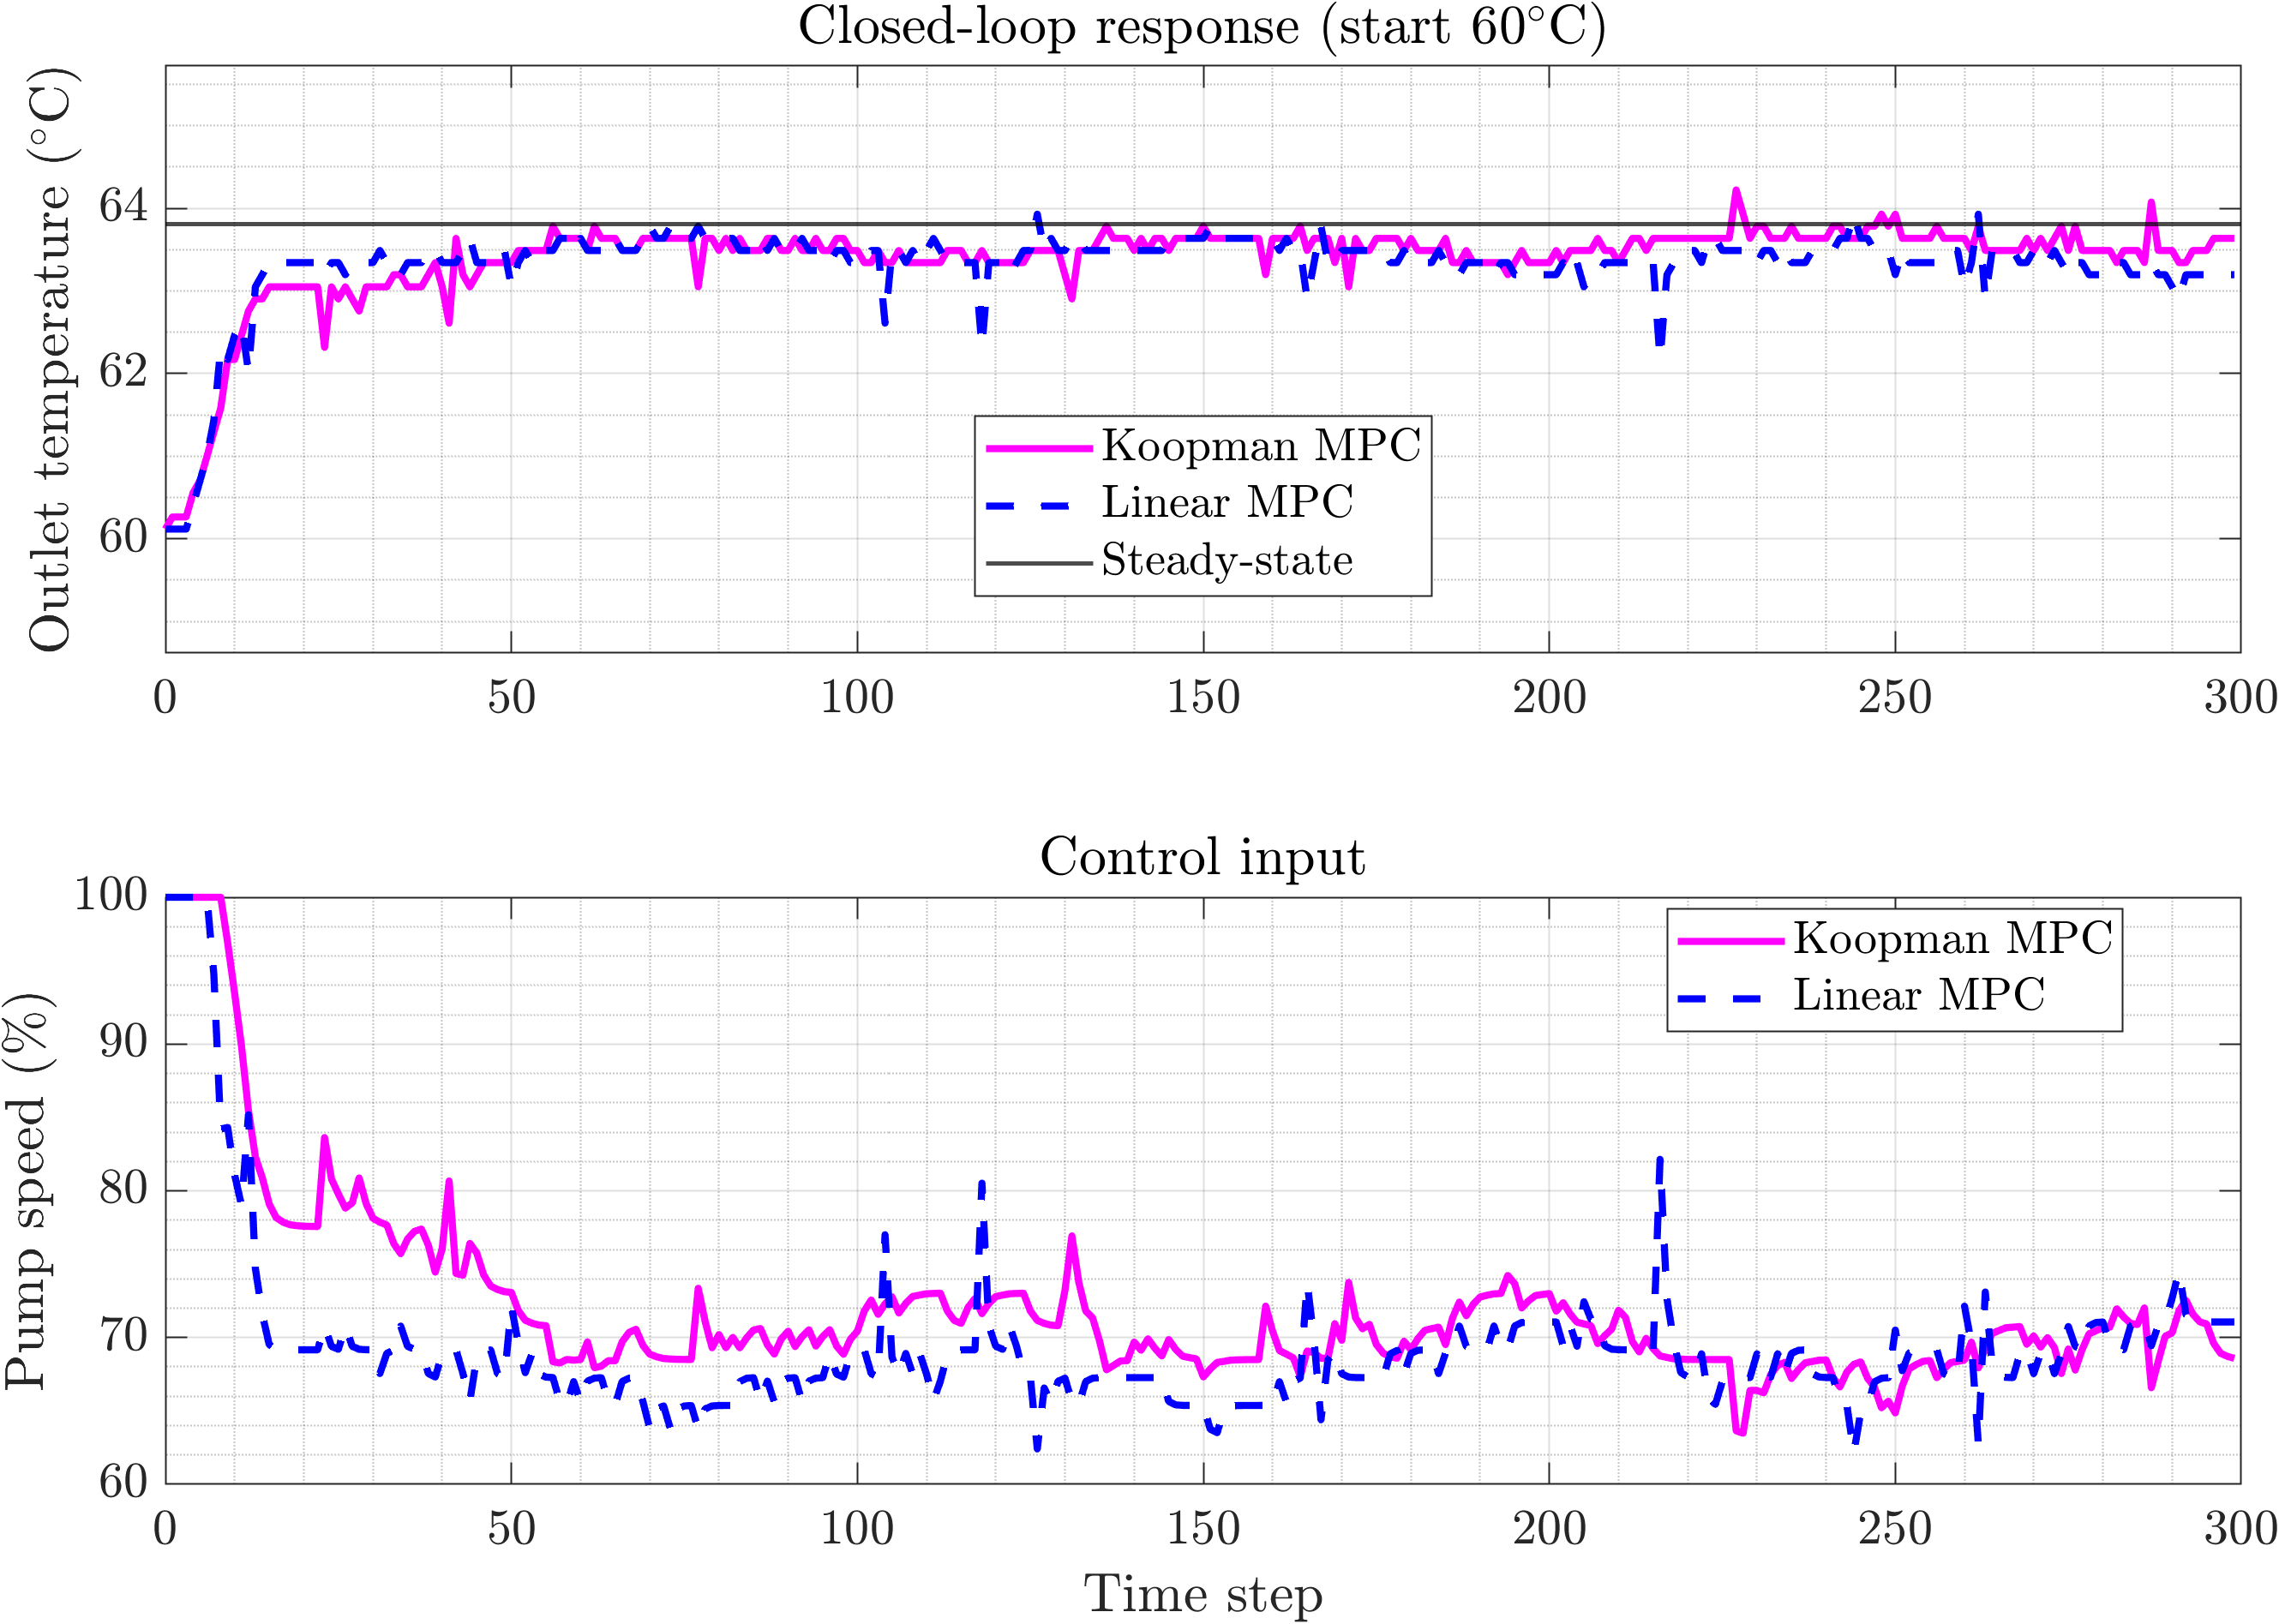
\includegraphics[width=\textwidth]{images/compare_cl_T0_60.png}
\caption{Closed-loop response and control input for $T_0 = 60\,^\circ\mathrm{C}$ with indicated settling time.}
\label{fig:cl_exp_T0_60}
\end{figure}

Both controllers
bring the temperature close to the steady-state with a small steady-state error.
The response comes from a real experiment executed sequentially, which results in small differences in the measured temperature.
At the beginning, the Koopman MPC keeps the input at the upper limit a bit
longer. Afterward, it decreases the input less aggressively than the linear MPC. The linear-model-based MPC reduces the input sooner and more aggressively,
and the temperature approaches the higher temperature steady-state more slowly. In this instance, the Koopman MPC leads
to a faster approach toward the steady-state.


The evaluation was performed for six initial temperatures in the range
$T_0 \in [55, 68]\,^\circ\mathrm{C}$. The resulting transient metrics for each case are summarized in Table~\ref{tab:transient_per_T0}, and is also visualized in Figure~\ref{fig:transient_metrics_summary}. 


\begin{table}[!t]
\centering
\caption{Transient performance metrics for Koopman MPC and linear-model-based MPC evaluated for different initial temperatures.}
\label{tab:transient_per_T0}
\resizebox{\textwidth}{!}{%
\begin{tabular}{c|ccccc|ccccc}
\hline
\multirow{2}{*}{$T_0$ [$^\circ$C]} &
\multicolumn{5}{c|}{Koopman MPC} &
\multicolumn{5}{c}{Linear MPC} \\
&
$T_s$ & IAE & ISE & ITAE & $J_{\mathrm{CL}}$ &
$T_s$ & IAE & ISE & ITAE & $J_{\mathrm{CL}}$ \\
\hline
55 & 69 & 228.465 & 1189.917 & 4463.122  & 358.001 &
65 & 208.862 & 1013.379 & 4075.616  & 304.534 \\
58 & 59 & 135.638 & 465.967  & 2394.468  & 180.042 &
75 & 173.925 & 612.048  & 3824.761  & 213.544 \\
60 & 51 & 62.025  & 121.280  & 1004.806  & 60.724  &
54 & 53.157  & 109.885  & 782.014   & 43.973 \\
% \rowcolor{gray!15}
62 & 12 & 16.166  & 23.689   & 72.070    & 20.112  &
299 & 225.071 & 190.701  & 31304.541 & 74.605 \\
66 & 69 & 54.526  & 63.489   & 1362.098  & 38.671  &
36 & 30.342  & 41.200   & 379.695   & 26.504 \\
68 & 62 & 70.704  & 156.091  & 1355.801  & 78.220  &
63 & 71.834  & 142.957  & 1558.893  & 78.319 \\
\hline
\textbf{Mean} &
53.67 & 94.59  & 336.74 & 1775.39 & 122.63 &
98.67 & 127.20 & 351.69 & 6987.59 & 123.58 \\
\textbf{Sum} &
322 & 567.52 & 2020.43 & 10652.37 & 735.77 &
592 & 763.19 & 2110.17 & 41925.52 & 741.48 \\
\hline
\end{tabular}%
}
\end{table}

The integral metrics (IAE, ISE, ITAE) are not
normalized by the duration of the transient phase. Consequently, their values depend not
only on the magnitude of the tracking error but also on the length of the transient phase.
For this reason, these metrics should be
interpreted in conjunction with the settling time.



The results indicate that both controllers provide comparable transient
performance; however, neither controller demonstrates uniformly superior performance across all initial
conditions. Overall, the Koopman MPC achieves shorter settling times
and lower accumulated error, especially in terms of IAE and ITAE. On average, the Koopman MPC achieves a substantially shorter settling time
($53.67$ samples compared to $98.67$ samples) and lower mean IAE
($94.59$ compared to $127.20$). The mean values of ISE and the transient
objective function are very similar for both controllers.

For illustration, take $T_0 = 62,^\circ\mathrm{C}$, where the Koopman MPC reaches the settling band after only $12$ samples, while the linear model-based MPC does not satisfy the settling condition until the end of the observation window. Consequently, the integral-based metrics for the linear MPC become considerably larger, primarily due to the longer transient duration.


\begin{figure}[!t]
    \centering
    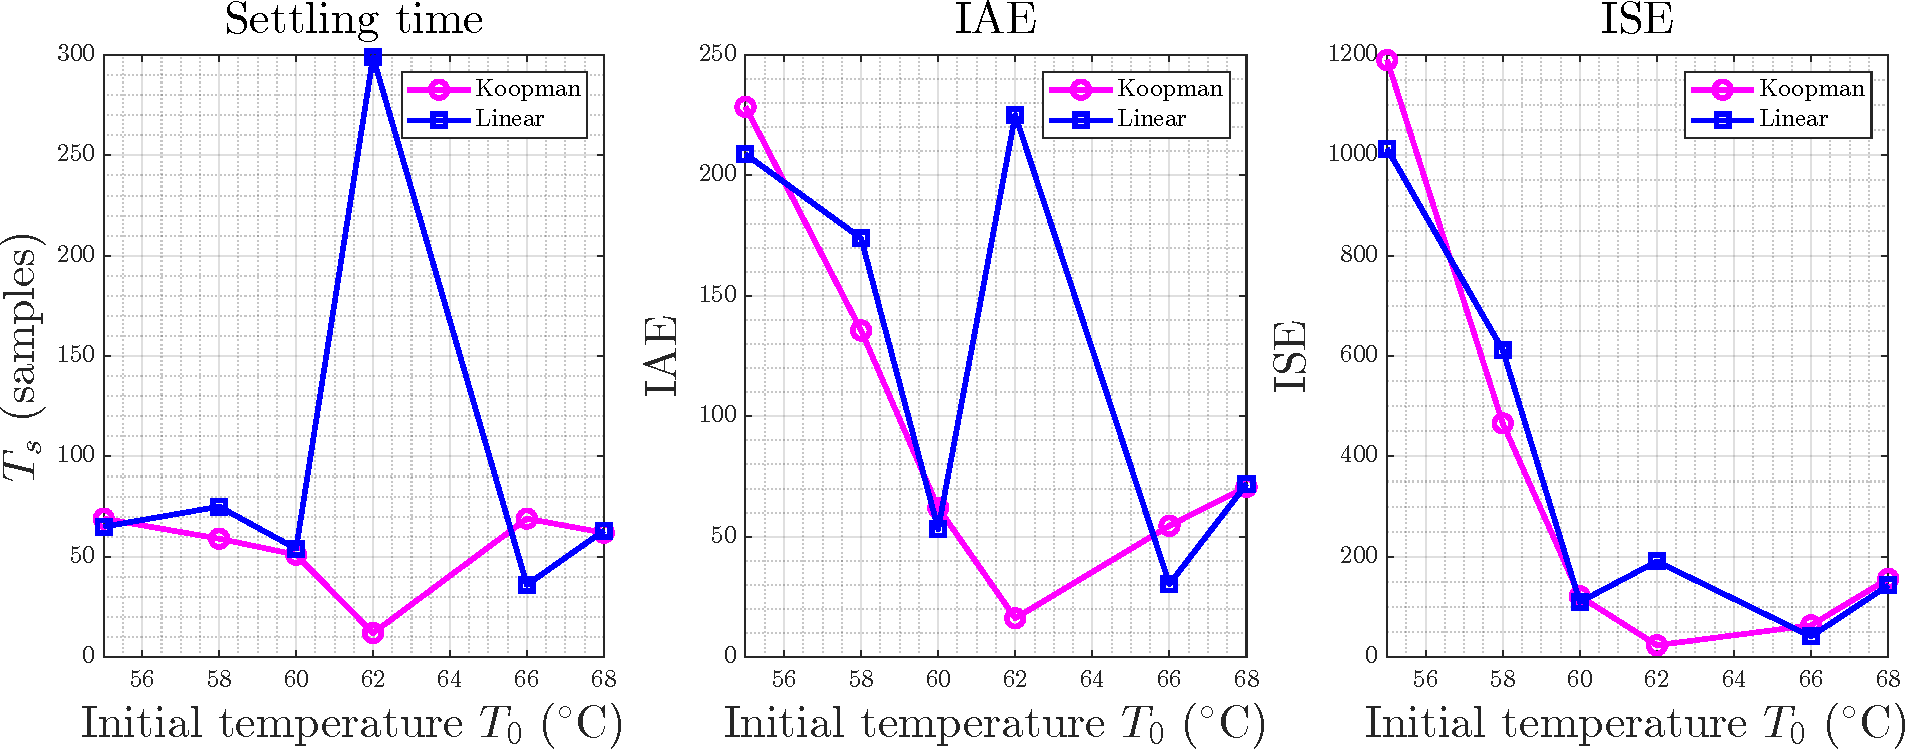
\includegraphics[width=\linewidth]{images/transient_metrics_summary_1.pdf}

    \vspace{0.8em}

    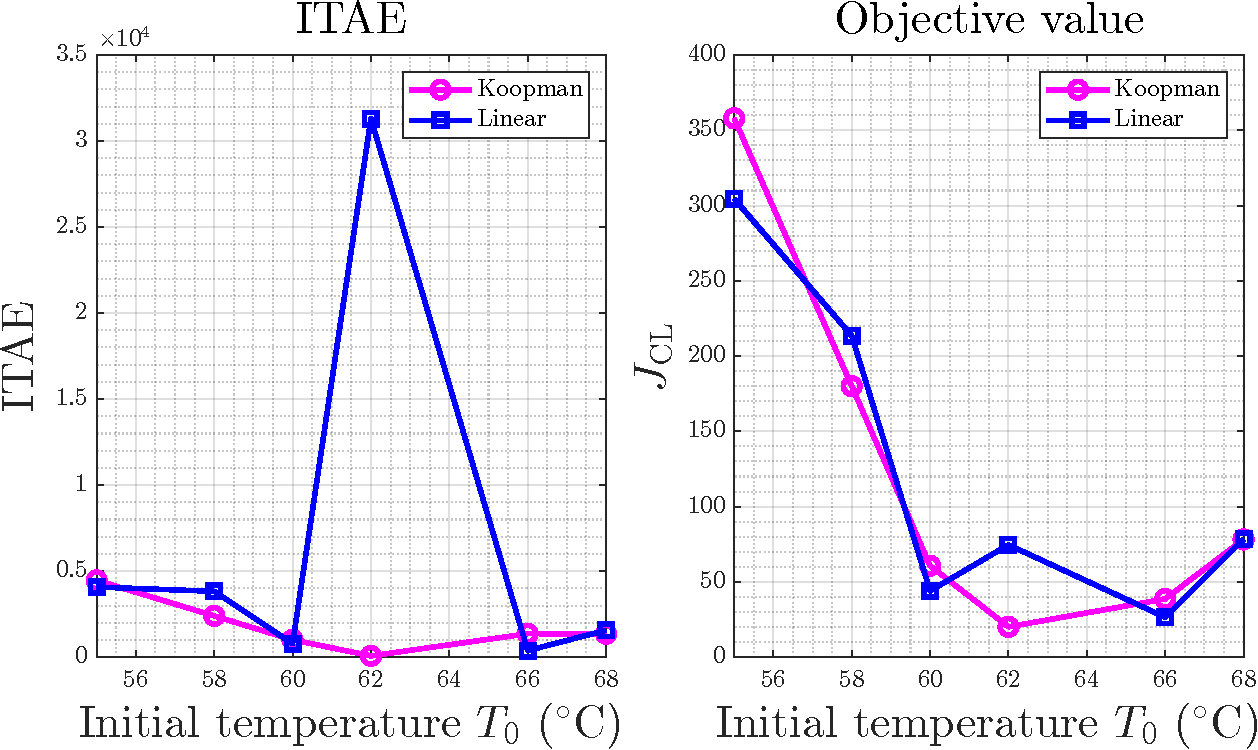
\includegraphics[width=0.67\linewidth]{images/transient_metrics_summary_2.pdf}

    \caption{Transient performance metrics versus initial temperature $T_0$ for Koopman MPC and linear MPC: settling time $T_s$, IAE, ISE, ITAE, and the transient objective value $J_{\mathrm{CL}}$.}
    \label{fig:transient_metrics_summary}
\end{figure}




\section{Discussion}
\label{sec:discussion}

This section discusses the main observations from the comparison of linear and Koopman-based MPC for plate heat exchanger control. The discussion focuses on the relation between model structure, closed-loop behavior, and practical applicability.

Both the first-order linear model and the data-driven Koopman model were identified from experimental data, but each model represents the process in a different way. The linear model captured the dominant thermal dynamics with a simple first-order structure, which made the controller design straightforward and provided reliable behavior near the operating point~\cite{ljung_sysid}. However, this model represents only a simplified approximation of the heat exchanger dynamics. Its accuracy therefore decreases when the system moves farther from the operating region or when nonlinear heat-transfer effects and disturbances become more significant. This was also visible in open-loop prediction, where the linear model showed accumulated prediction errors over longer horizons, with an open-loop RMSE of approximately $1.70\,^\circ$C.

The Koopman model used neural-network-based lifting to represent the measured dynamics in a higher-dimensional latent space. This gave the model more flexibility and allowed it to approximate nonlinear input--output behavior better than the first-order linear model~\cite{korda2018, otto2019linearly, yeung2019learning}. The open-loop prediction error was slightly lower, with an RMSE of approximately $1.67\,^\circ$C. This improvement is not large, but it may indicate that the lifted representation captures additional information about the process dynamics. At the same time, this increased flexibility requires more data, computational resources, as discussed in Section~\ref{sec:koopman_identification}, and may benefit from more careful tuning. Since no explicit stability constraint was imposed during training, the generalization of the model outside the identified operating region remains an important limitation.

The closed-loop behavior follows directly from the model properties. The linear MPC is based on a conservative prediction model that mainly describes the dominant slow thermal response of the heat exchanger. As a result, it usually produces smoother and more regular control inputs. The Koopman MPC, on the other hand, uses a prediction model that can represent nonlinear transient behavior more flexibly. It reacts more strongly when the measured temperature differs from the desired operating region. This explains why the Koopman controller often reduces the tracking error faster, but may also produce more aggressive input changes or small overshoots.

Both controllers were implemented with identical structure, constraints, and weights, as described in Section~\ref{sec:mpc_design}. This allowed the effect of the prediction model to be compared under the same control design. However, identical tuning is not necessarily optimal for both models. The linear controller might benefit from more conservative tuning, while the Koopman controller could potentially use its more expressive prediction model more effectively with different weights or additional constraints on the input movement.

The simulation results in Section~\ref{sec:simulation_results} showed that both controllers achieved stable regulation of the nonlinear baseline plant. The Koopman MPC achieved slightly better mean tracking performance, with a mean RMSE of $1.59\,^\circ$C compared with $1.65\,^\circ$C for the linear MPC. The difference was small because the simulated plant was dominated by slow thermal dynamics and the tested operating range was not strongly nonlinear. Nevertheless, the Koopman controller consistently achieved lower accumulated error, which confirms that the lifted model provided a small advantage during transient responses.

The experimental results in Section~\ref{sec:experimental_results} showed the same main trend, but with more visible differences caused by real process effects. The real heat exchanger includes measurement noise, actuator limitations, hydraulic disturbances, and nonlinear heat-transfer behavior that are not fully represented in either model. Under these conditions, the Koopman MPC reached the settling band faster, with a mean settling time of $54$ samples compared with $99$ samples for the linear MPC, as shown in Table~\ref{tab:transient_per_T0}. This faster response is a result of the more responsive prediction model and stronger initial control actions. The linear MPC was smoother and sometimes achieved slightly lower objective values, especially near the operating point, because the closed-loop objective also penalizes control effort.

Overall, the results show that both controllers are suitable for predictive control of the plate heat exchanger. The linear MPC provides a simple, interpretable, and robust solution for operation near the identified working point. The Koopman MPC introduces higher modeling complexity, but improves transient behavior and reduces accumulated tracking error in both simulations and experiments. Therefore, the main benefit of the Koopman approach is not a dramatic improvement in every metric, but its ability to provide faster and more accurate transient regulation while preserving the same MPC structure. This shows that Koopman-based modeling is a useful extension of classical linear predictive control for nonlinear thermal systems, especially when improved transient performance is required.




\newpage
\section{Conclusions}

This work addressed the modeling and control of a plate heat exchanger using two predictive models within an MPC framework. A first-order linear model identified from step response data was compared with a data-driven Koopman model obtained from measured input--output data using neural-network-based lifting. Both models were used as prediction models in MPC controllers with identical structure, constraints, and tuning, which allowed a direct comparison of the influence of the prediction model.

The linear model provided a simple and interpretable approximation of the dominant thermal dynamics of the heat exchanger. It was sufficient for stable control near the operating point and produced smooth control actions. The Koopman model introduced a higher-dimensional lifted representation of the system and provided a more flexible data-driven description of the process dynamics. This increased model complexity, but also improved the representation of transient behavior.

Closed-loop simulations showed that both controllers were able to regulate the simulated nonlinear plant to the desired steady-state region. The differences between the controllers were relatively small, because the simulated process was dominated by slow thermal dynamics and operated within a limited range. Nevertheless, the Koopman-based MPC achieved slightly lower tracking errors and lower accumulated error in most tested cases.

The experimental results confirmed that both controllers can be applied to the real plate heat exchanger. The Koopman MPC generally reached the steady-state region faster and achieved lower accumulated transient errors. This was caused by a more responsive prediction model and stronger initial control actions. The linear MPC showed smoother and more conservative behavior, which sometimes resulted in slightly lower objective values when the control effort was also taken into account.

The results therefore show a clear trade-off between model simplicity and transient performance. The linear MPC is easier to identify, interpret, and implement, and it is suitable when smooth and robust behavior near the operating point is required. The Koopman-based MPC is more complex and requires more careful identification, but it can improve transient regulation and reduce accumulated tracking error.

In this work, the Koopman model was identified for a SISO configuration with a pump as the manipulated input and the outlet temperature as the controlled output. If the operating regime, input, or controlled variable changes significantly, the model should be re-identified using new measured data. However, the MPC formulation itself can remain unchanged, which is an important practical advantage of the Koopman-based approach.

Overall, the thesis demonstrates that Koopman-based MPC is a suitable extension of classical linear MPC for the control of nonlinear thermal systems. For the investigated plate heat exchanger, the improvement was most visible during the transient phase, where the Koopman controller achieved faster convergence and lower accumulated error while maintaining stable closed-loop behavior.
